\newpage
\section{RESULTS}

\subsection{Experimental Results}
The photographs were captured while analysing parameters related to wastewater and sludge, and some collected samples are shown below.


\begin{figure}[H]
\centering

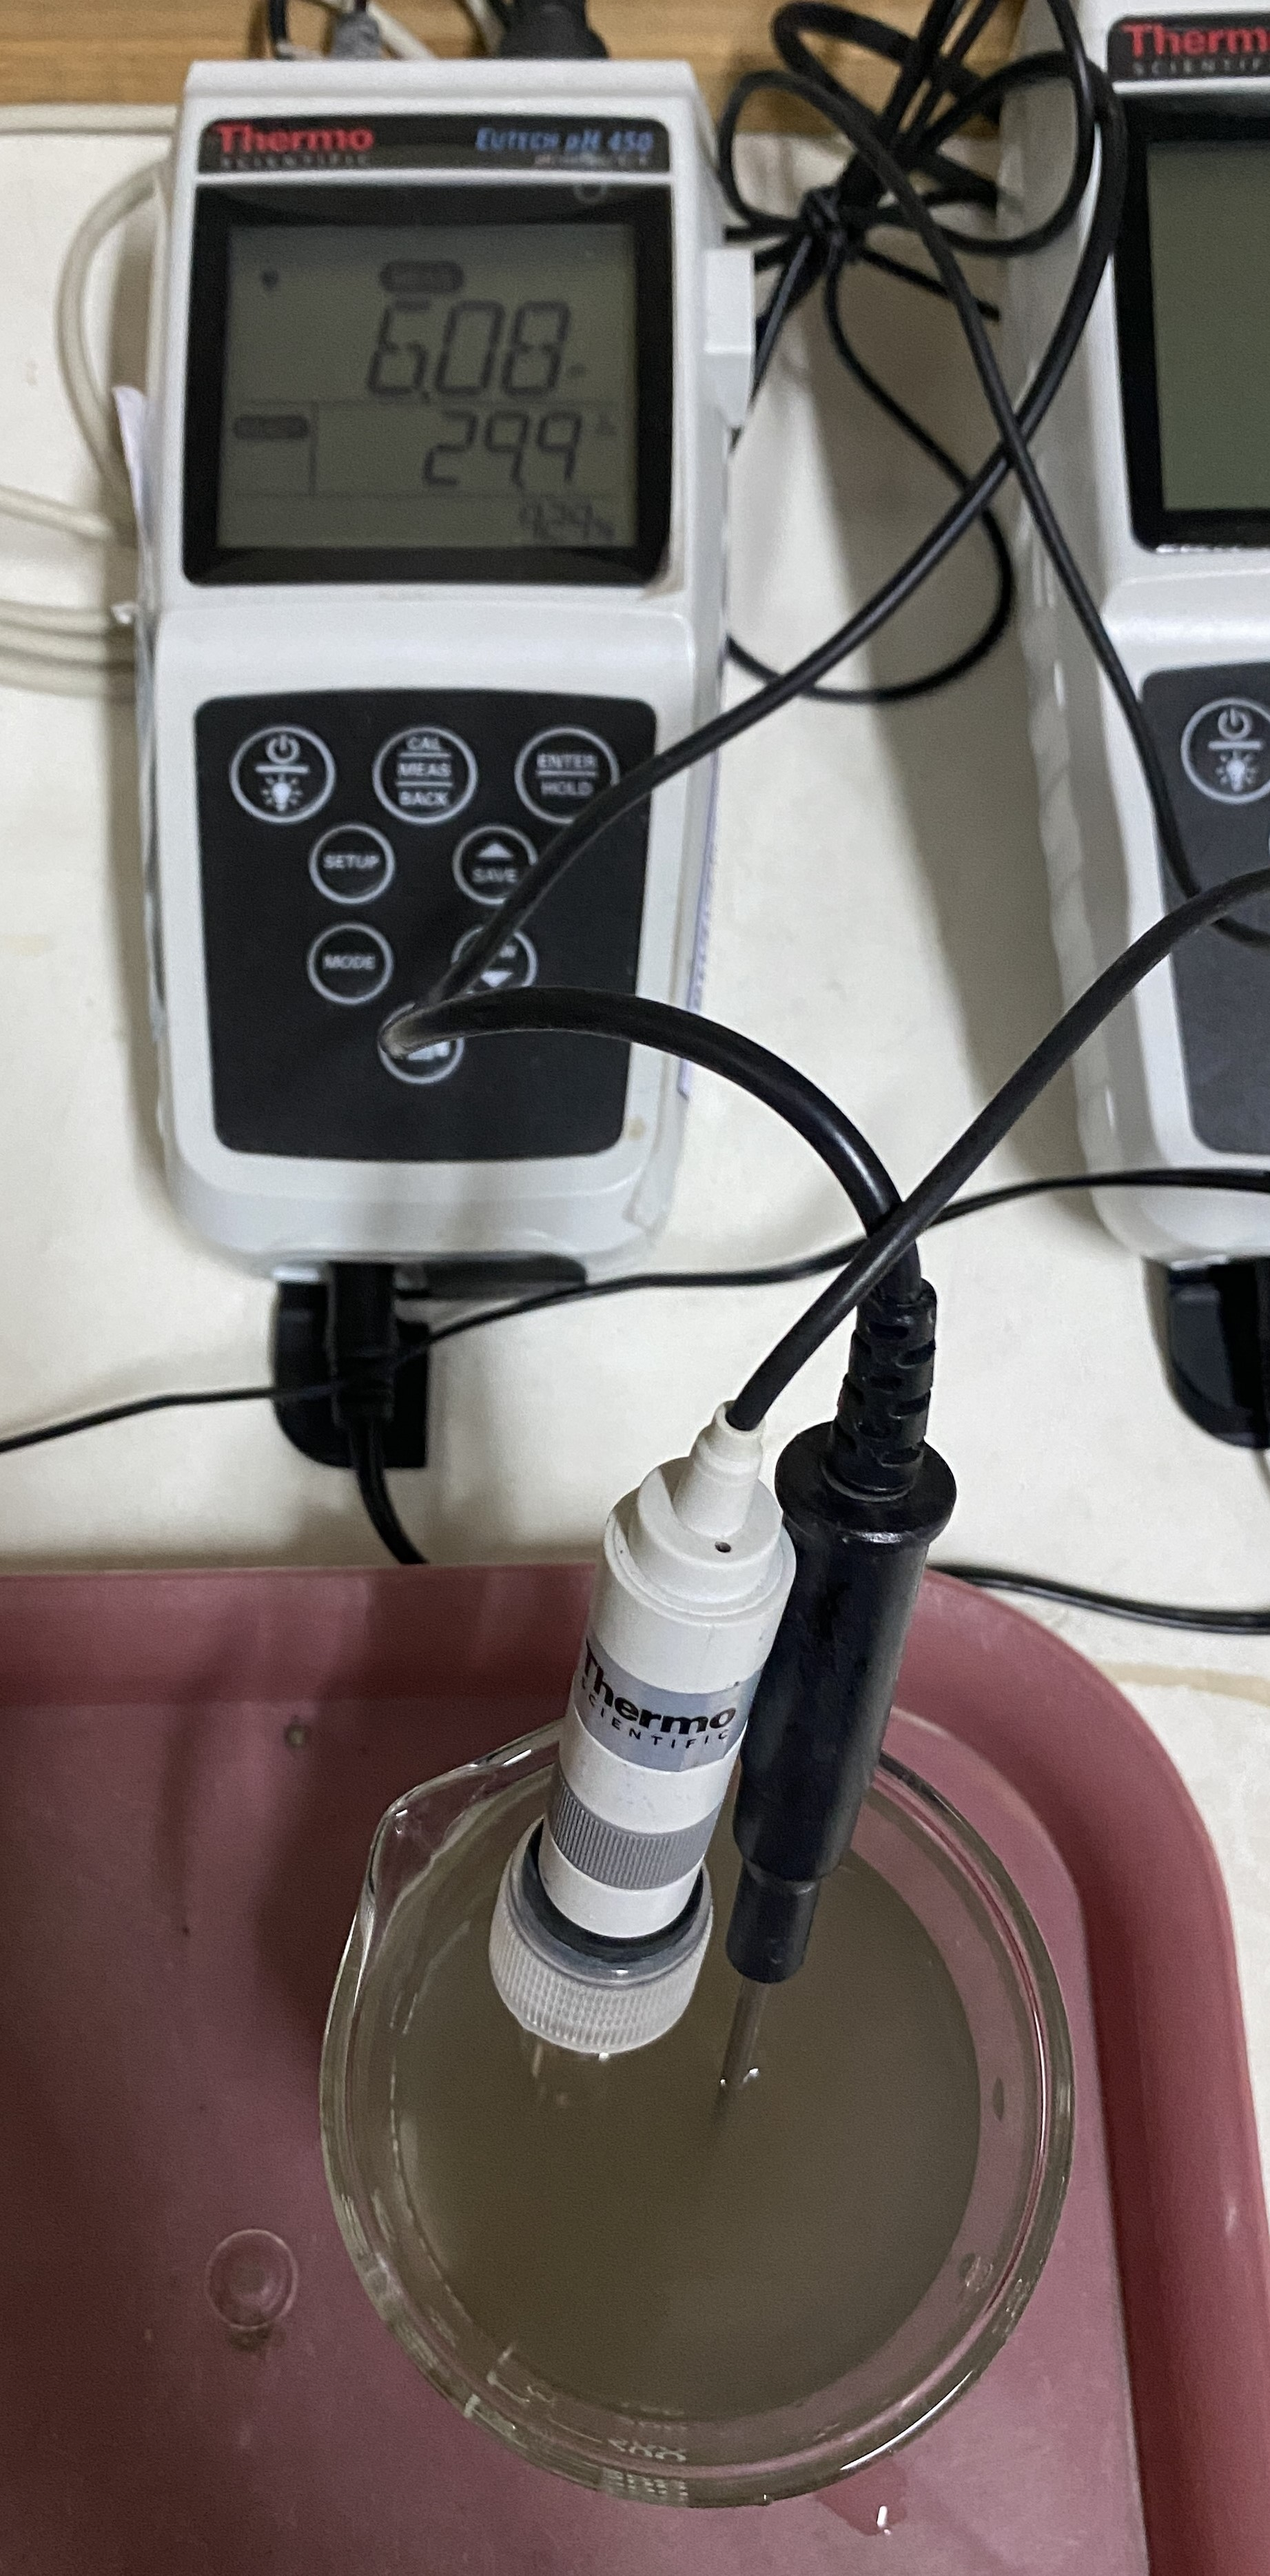
\includegraphics[width=.370\textwidth]{results/inlet_ph.JPG}\hfill
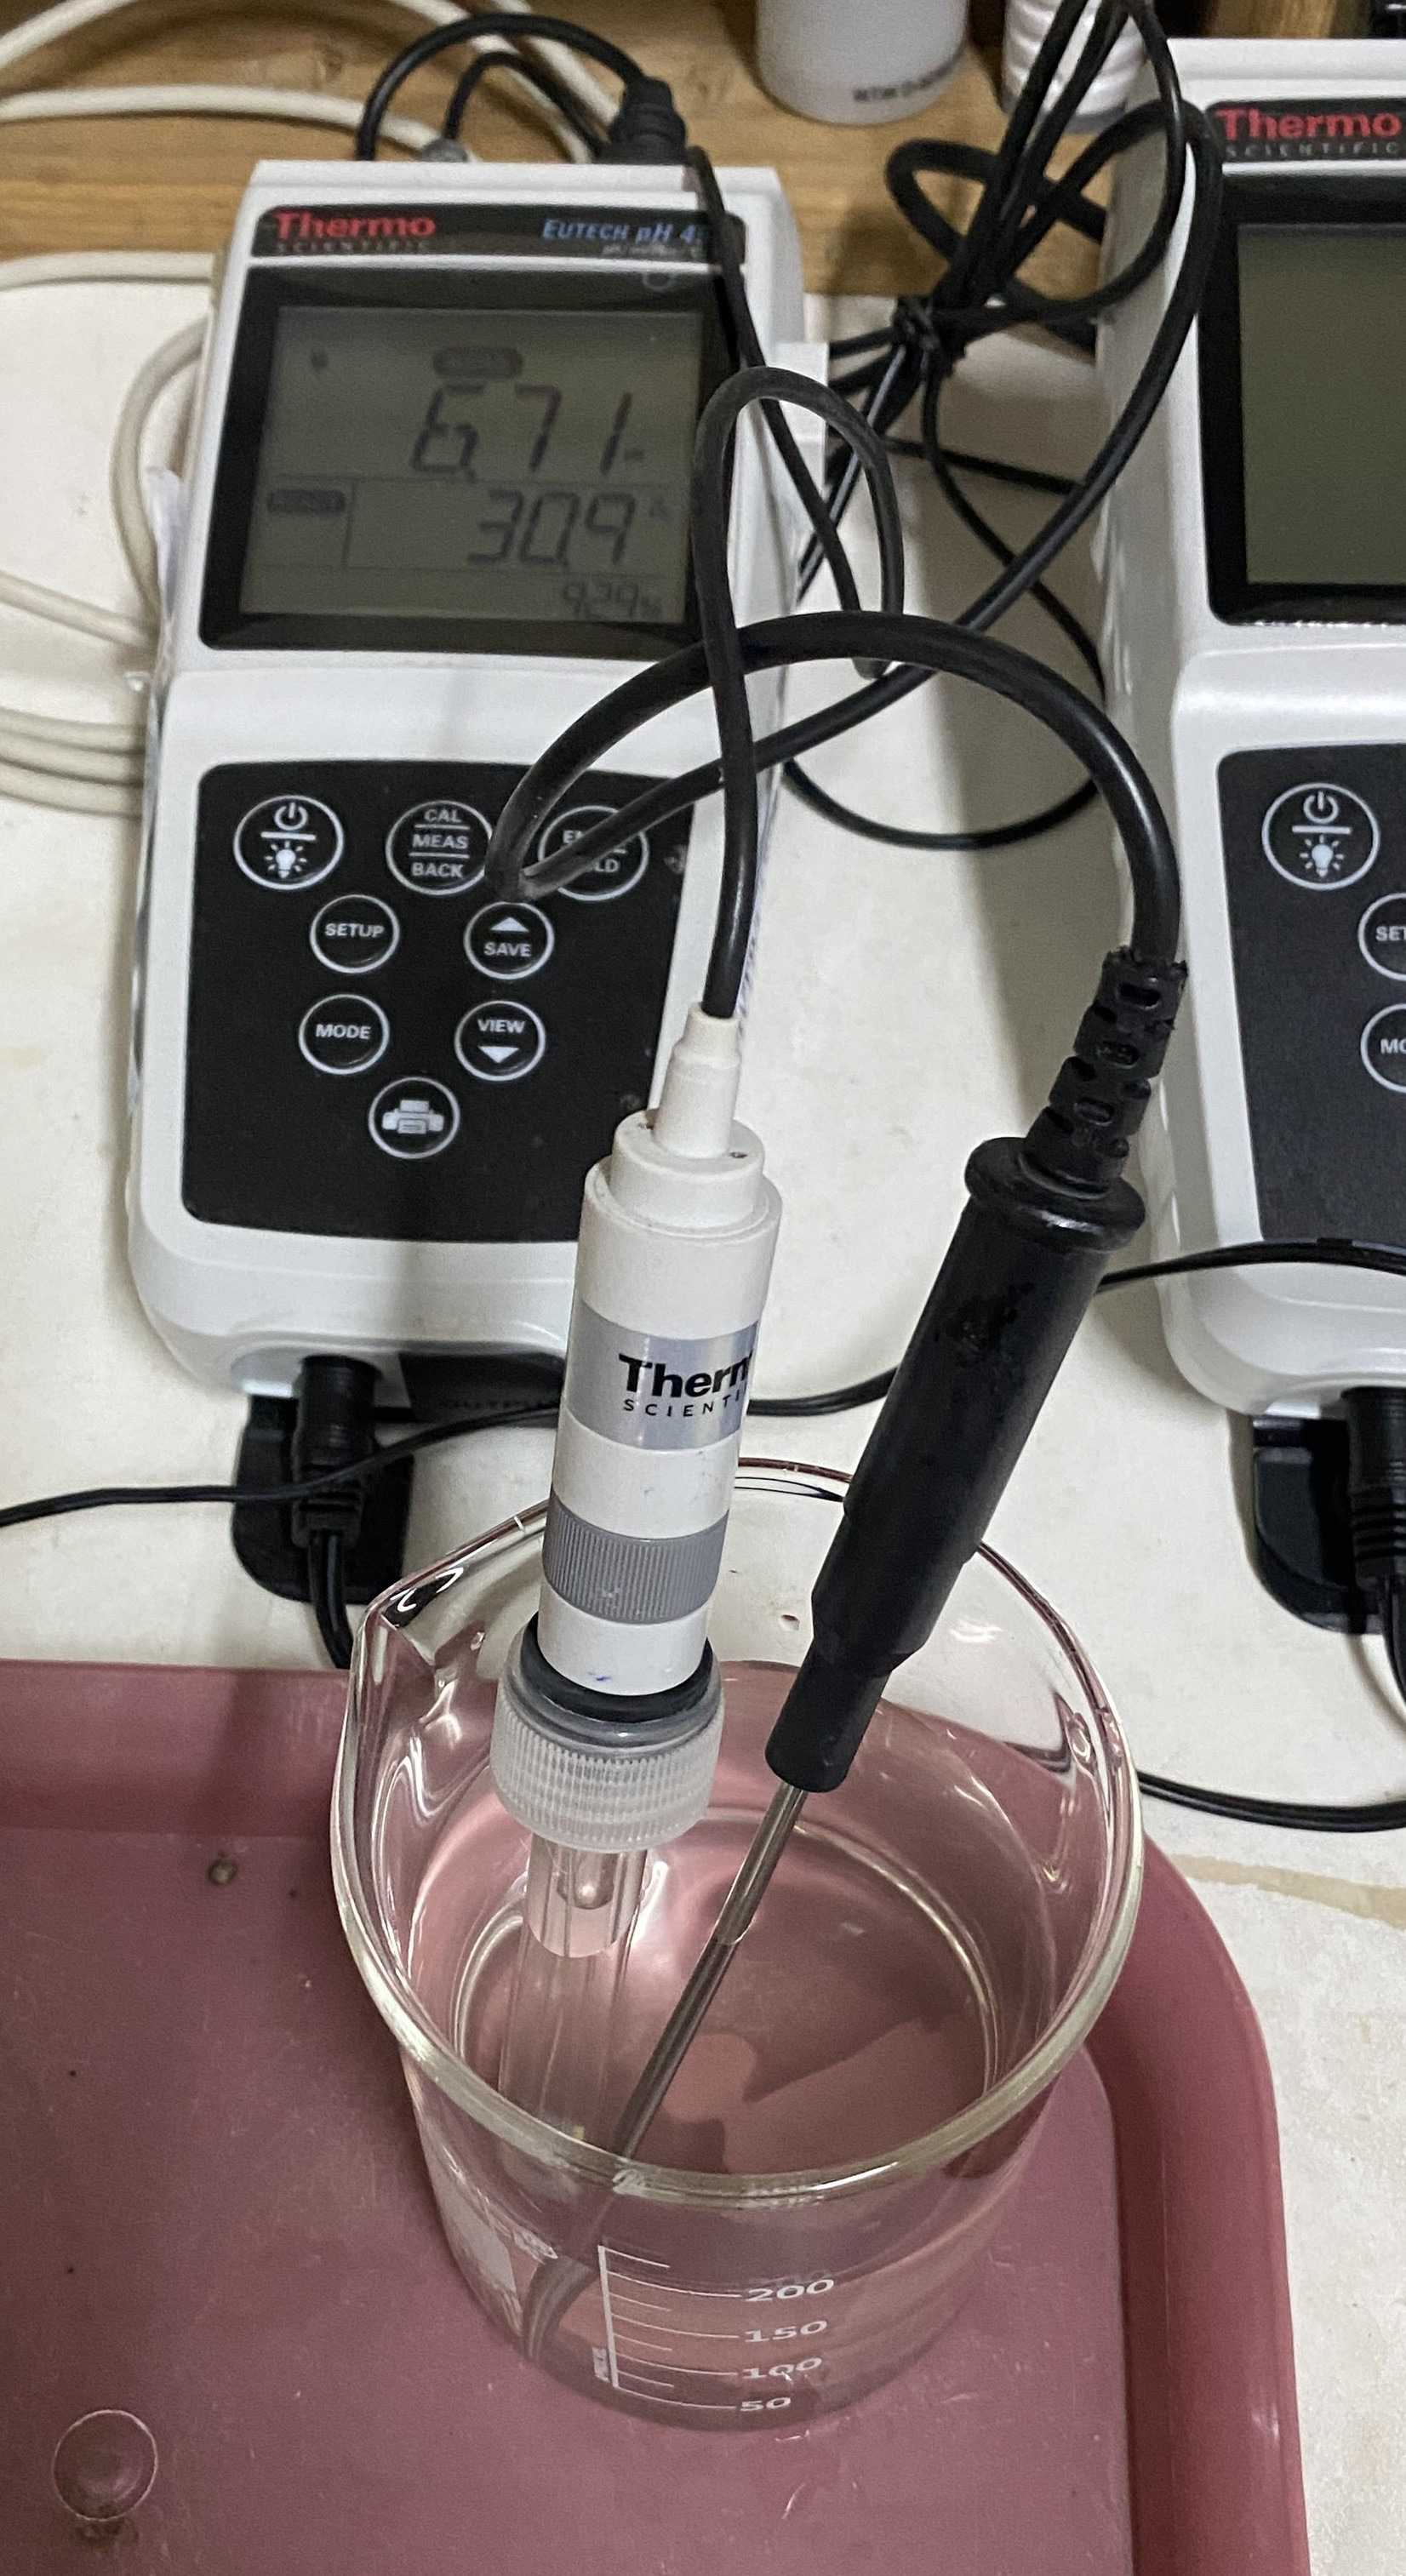
\includegraphics[width=.4\textwidth]{results/outlet_ph.JPG}\hfill

\caption{Measured pH and temperature of inlet and outlet}
\label{fig: pH and temperature}
\end{figure}


\begin{figure}[H]
\centering

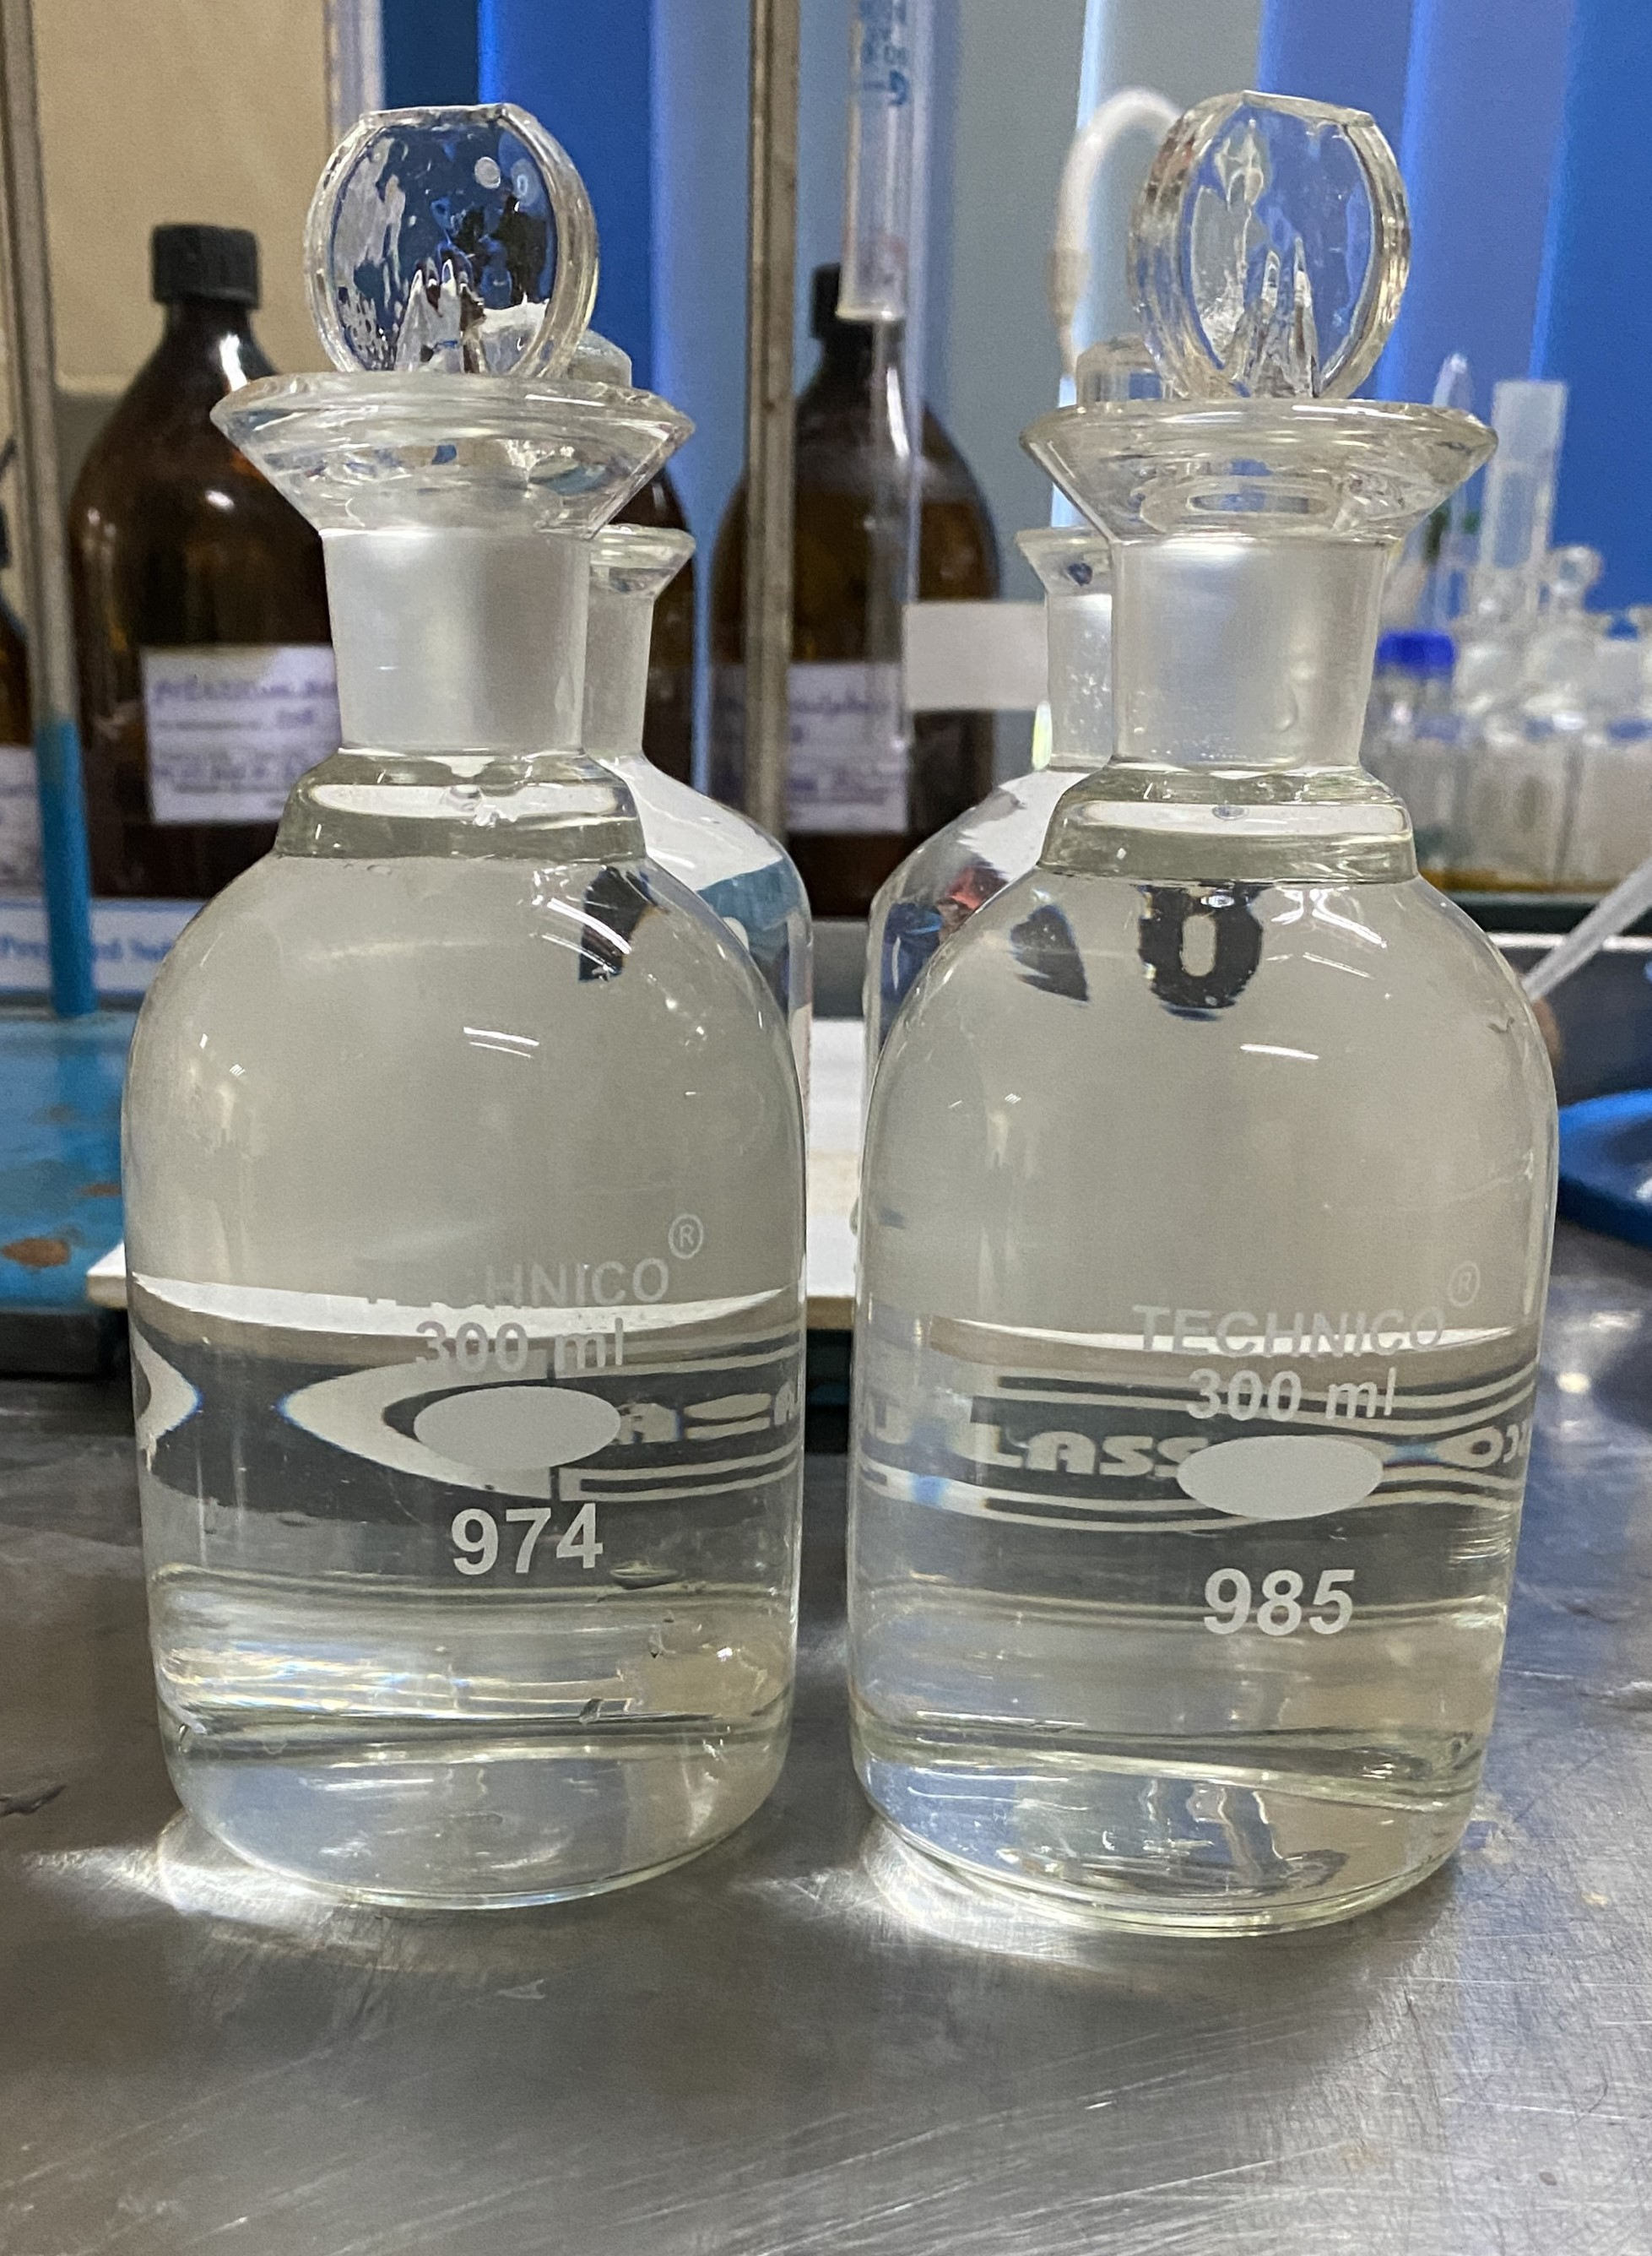
\includegraphics[width=.385\textwidth]{results/bod_before.JPG}\hfill
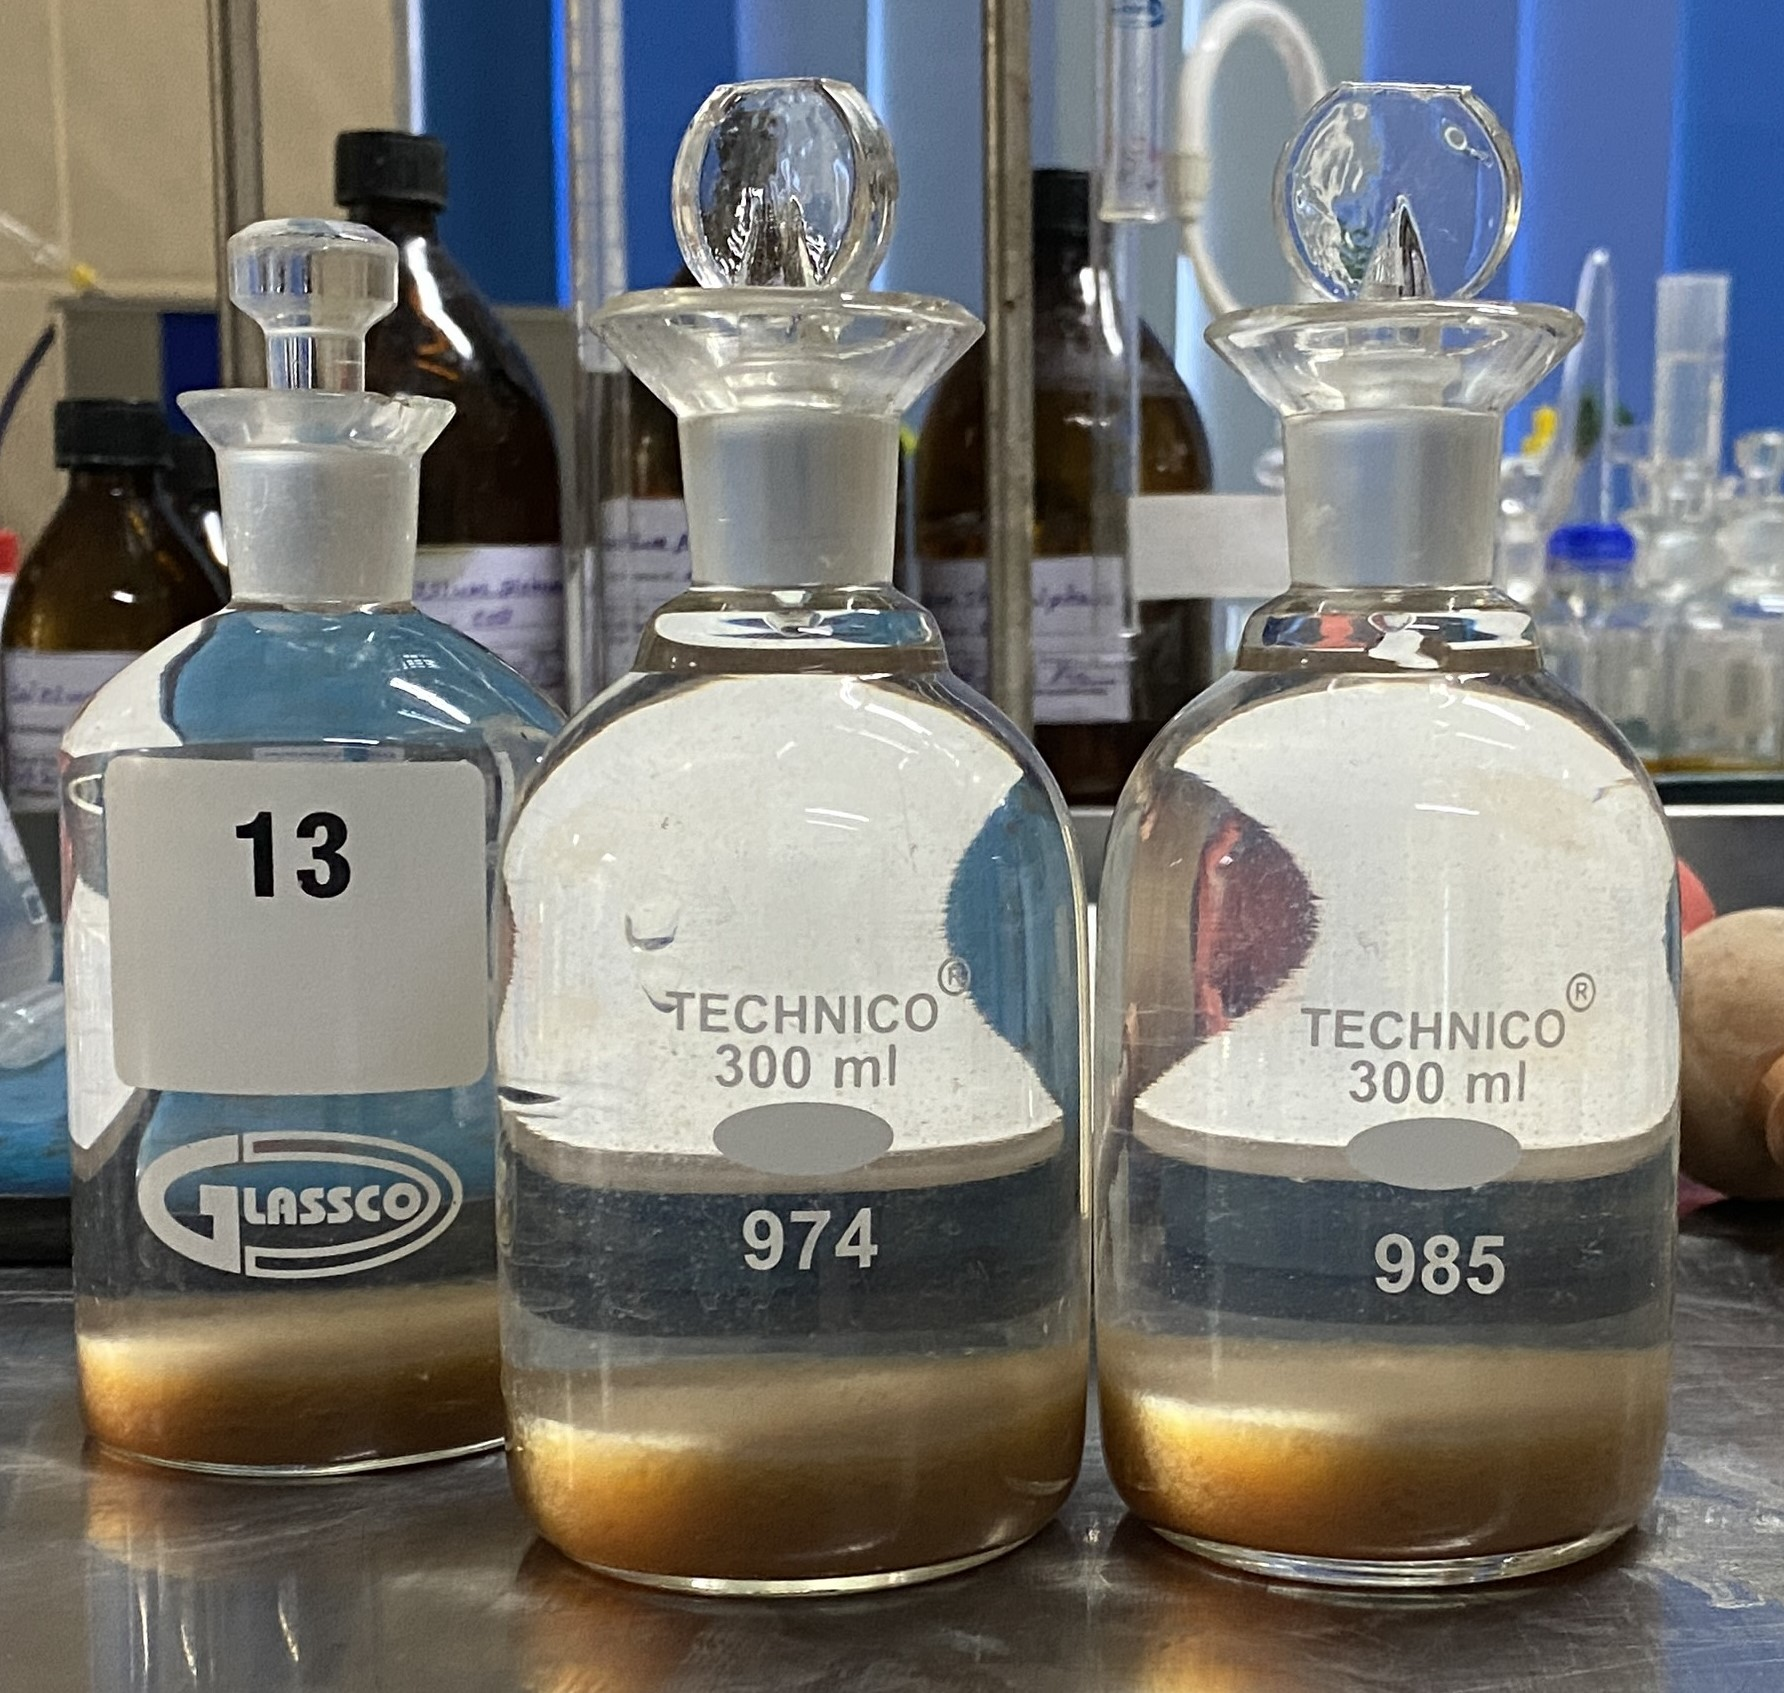
\includegraphics[width=.55\textwidth]{results/bod_precipitate.JPG}\hfill


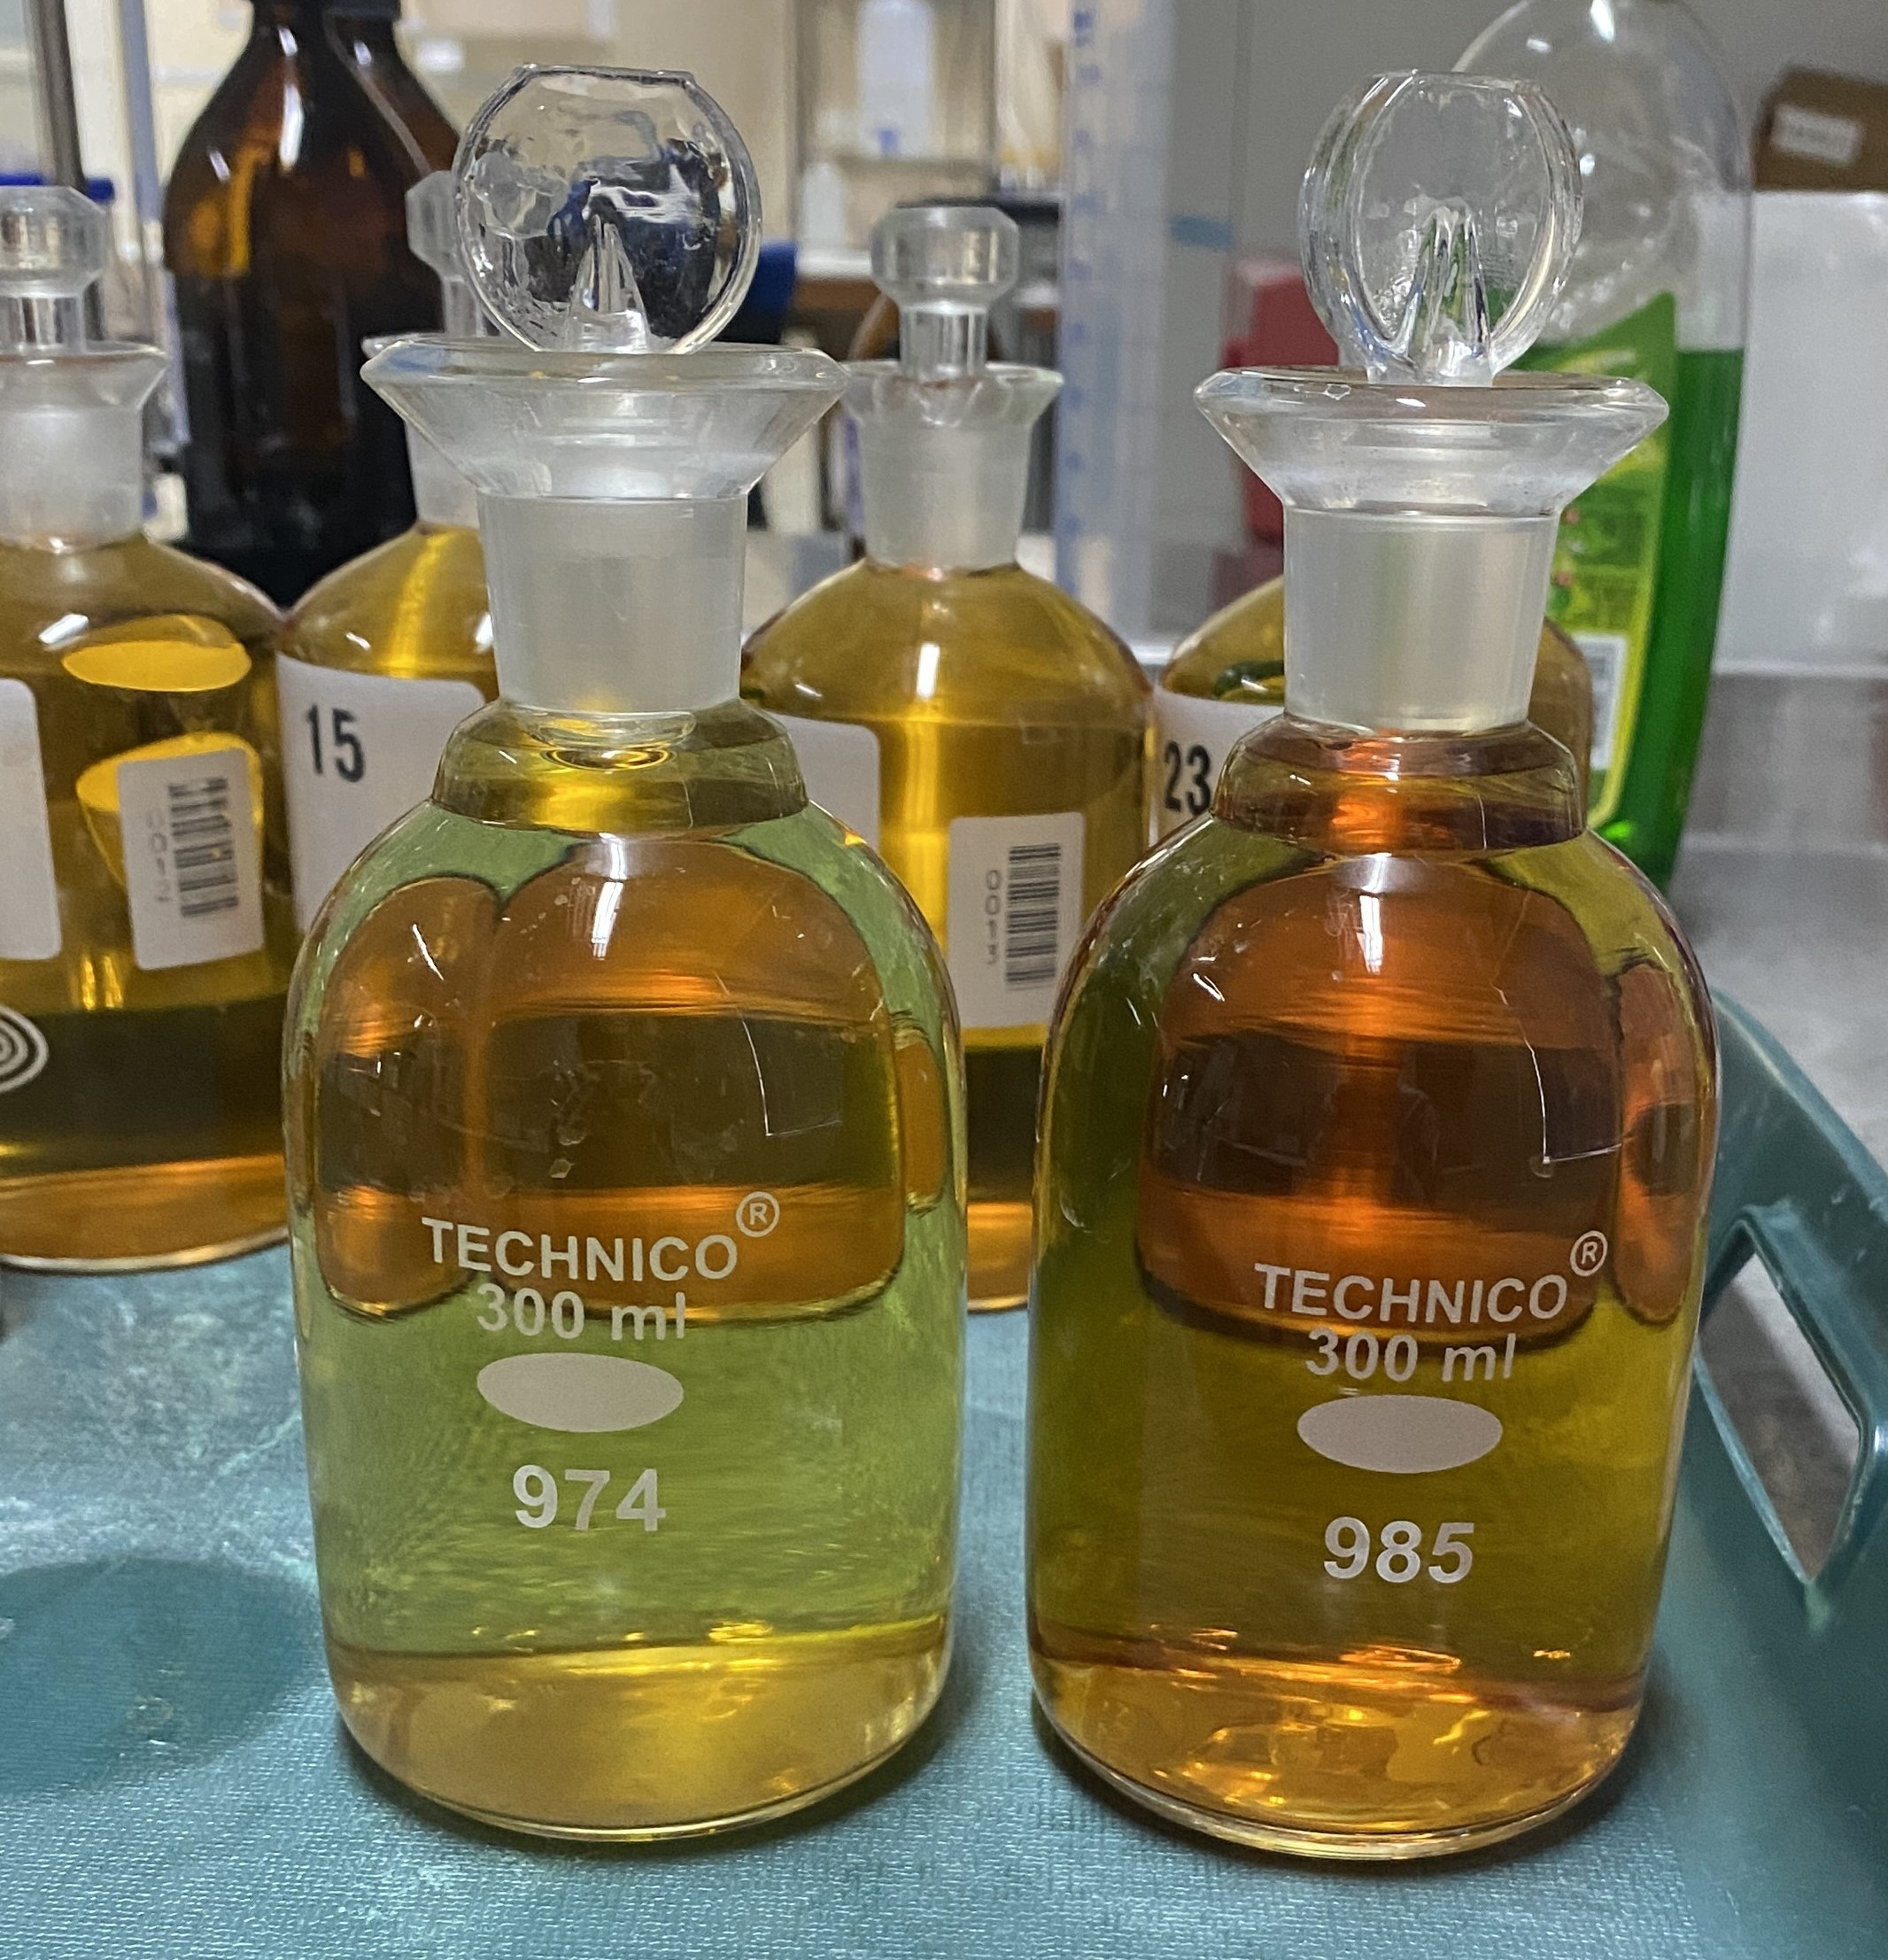
\includegraphics[width=.5\textwidth]{results/bod_after.JPG}\hfill


\caption{\ac{BOD5} analysed samples of inlet and outlet during 5 days}
\label{fig: bod_before_after_samples}
\end{figure}

\begin{figure}[H]
\centering

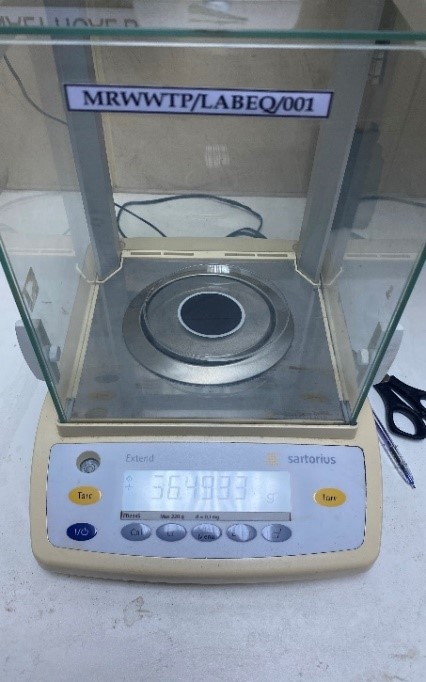
\includegraphics[width=.4\textwidth]{results/TSS.JPG}\hfill
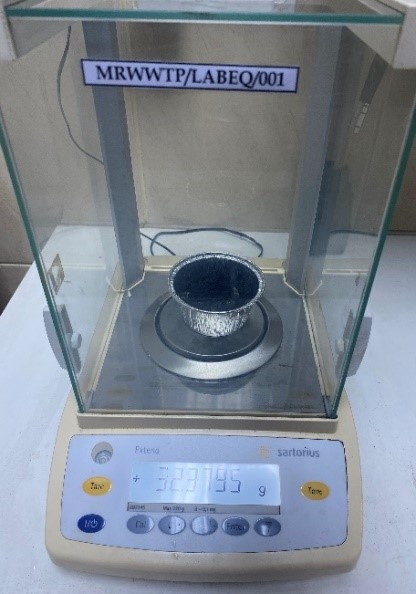
\includegraphics[width=.45\textwidth]{results/Dewatered sludge.jpg}\hfill

\caption{Measured weight of filtered paper for \ac{TSS} of the storage tank and the dried sludge sample }
\label{fig: TSS and Moisture content}
\end{figure}


\begin{figure}[H]
\centering
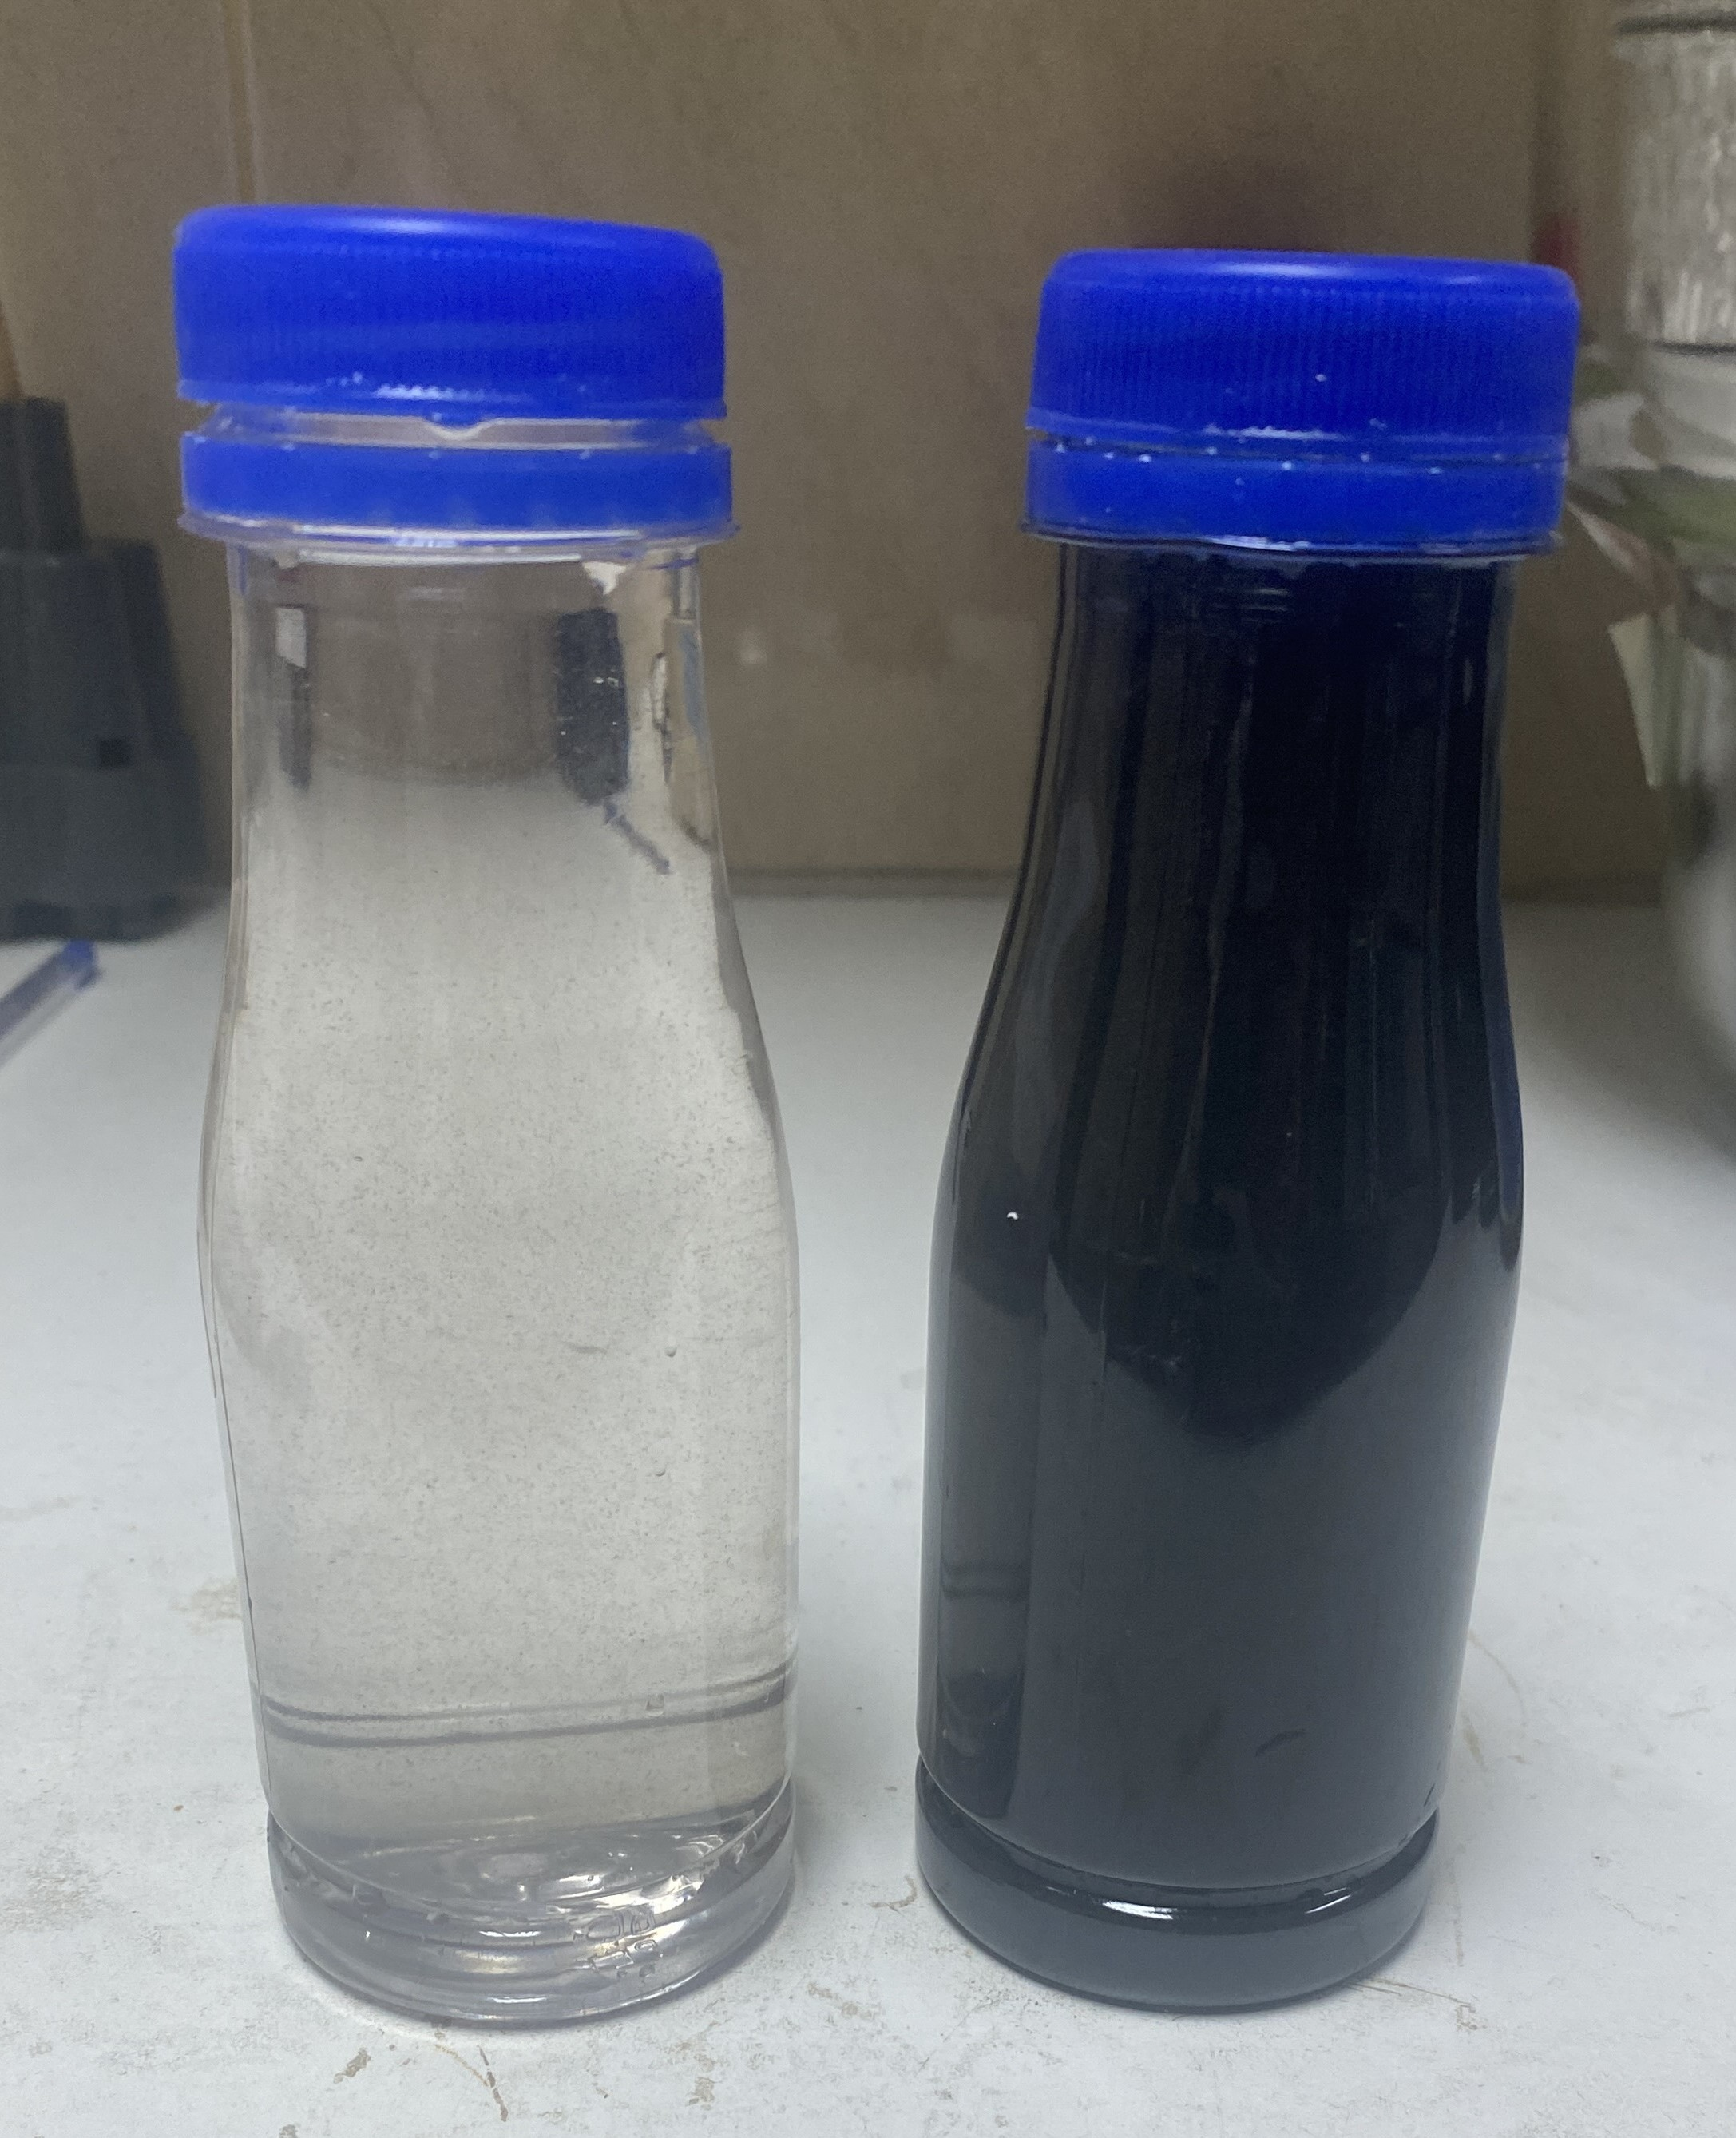
\includegraphics[width=0.4\linewidth]{results/Sample storage tank and return water.jpg}
\caption{Sample collected from the sludge storage tank and return water}
\label{fig:Sample_storagetank_returnwater}
\end{figure}

\begin{figure}[H]
\centering
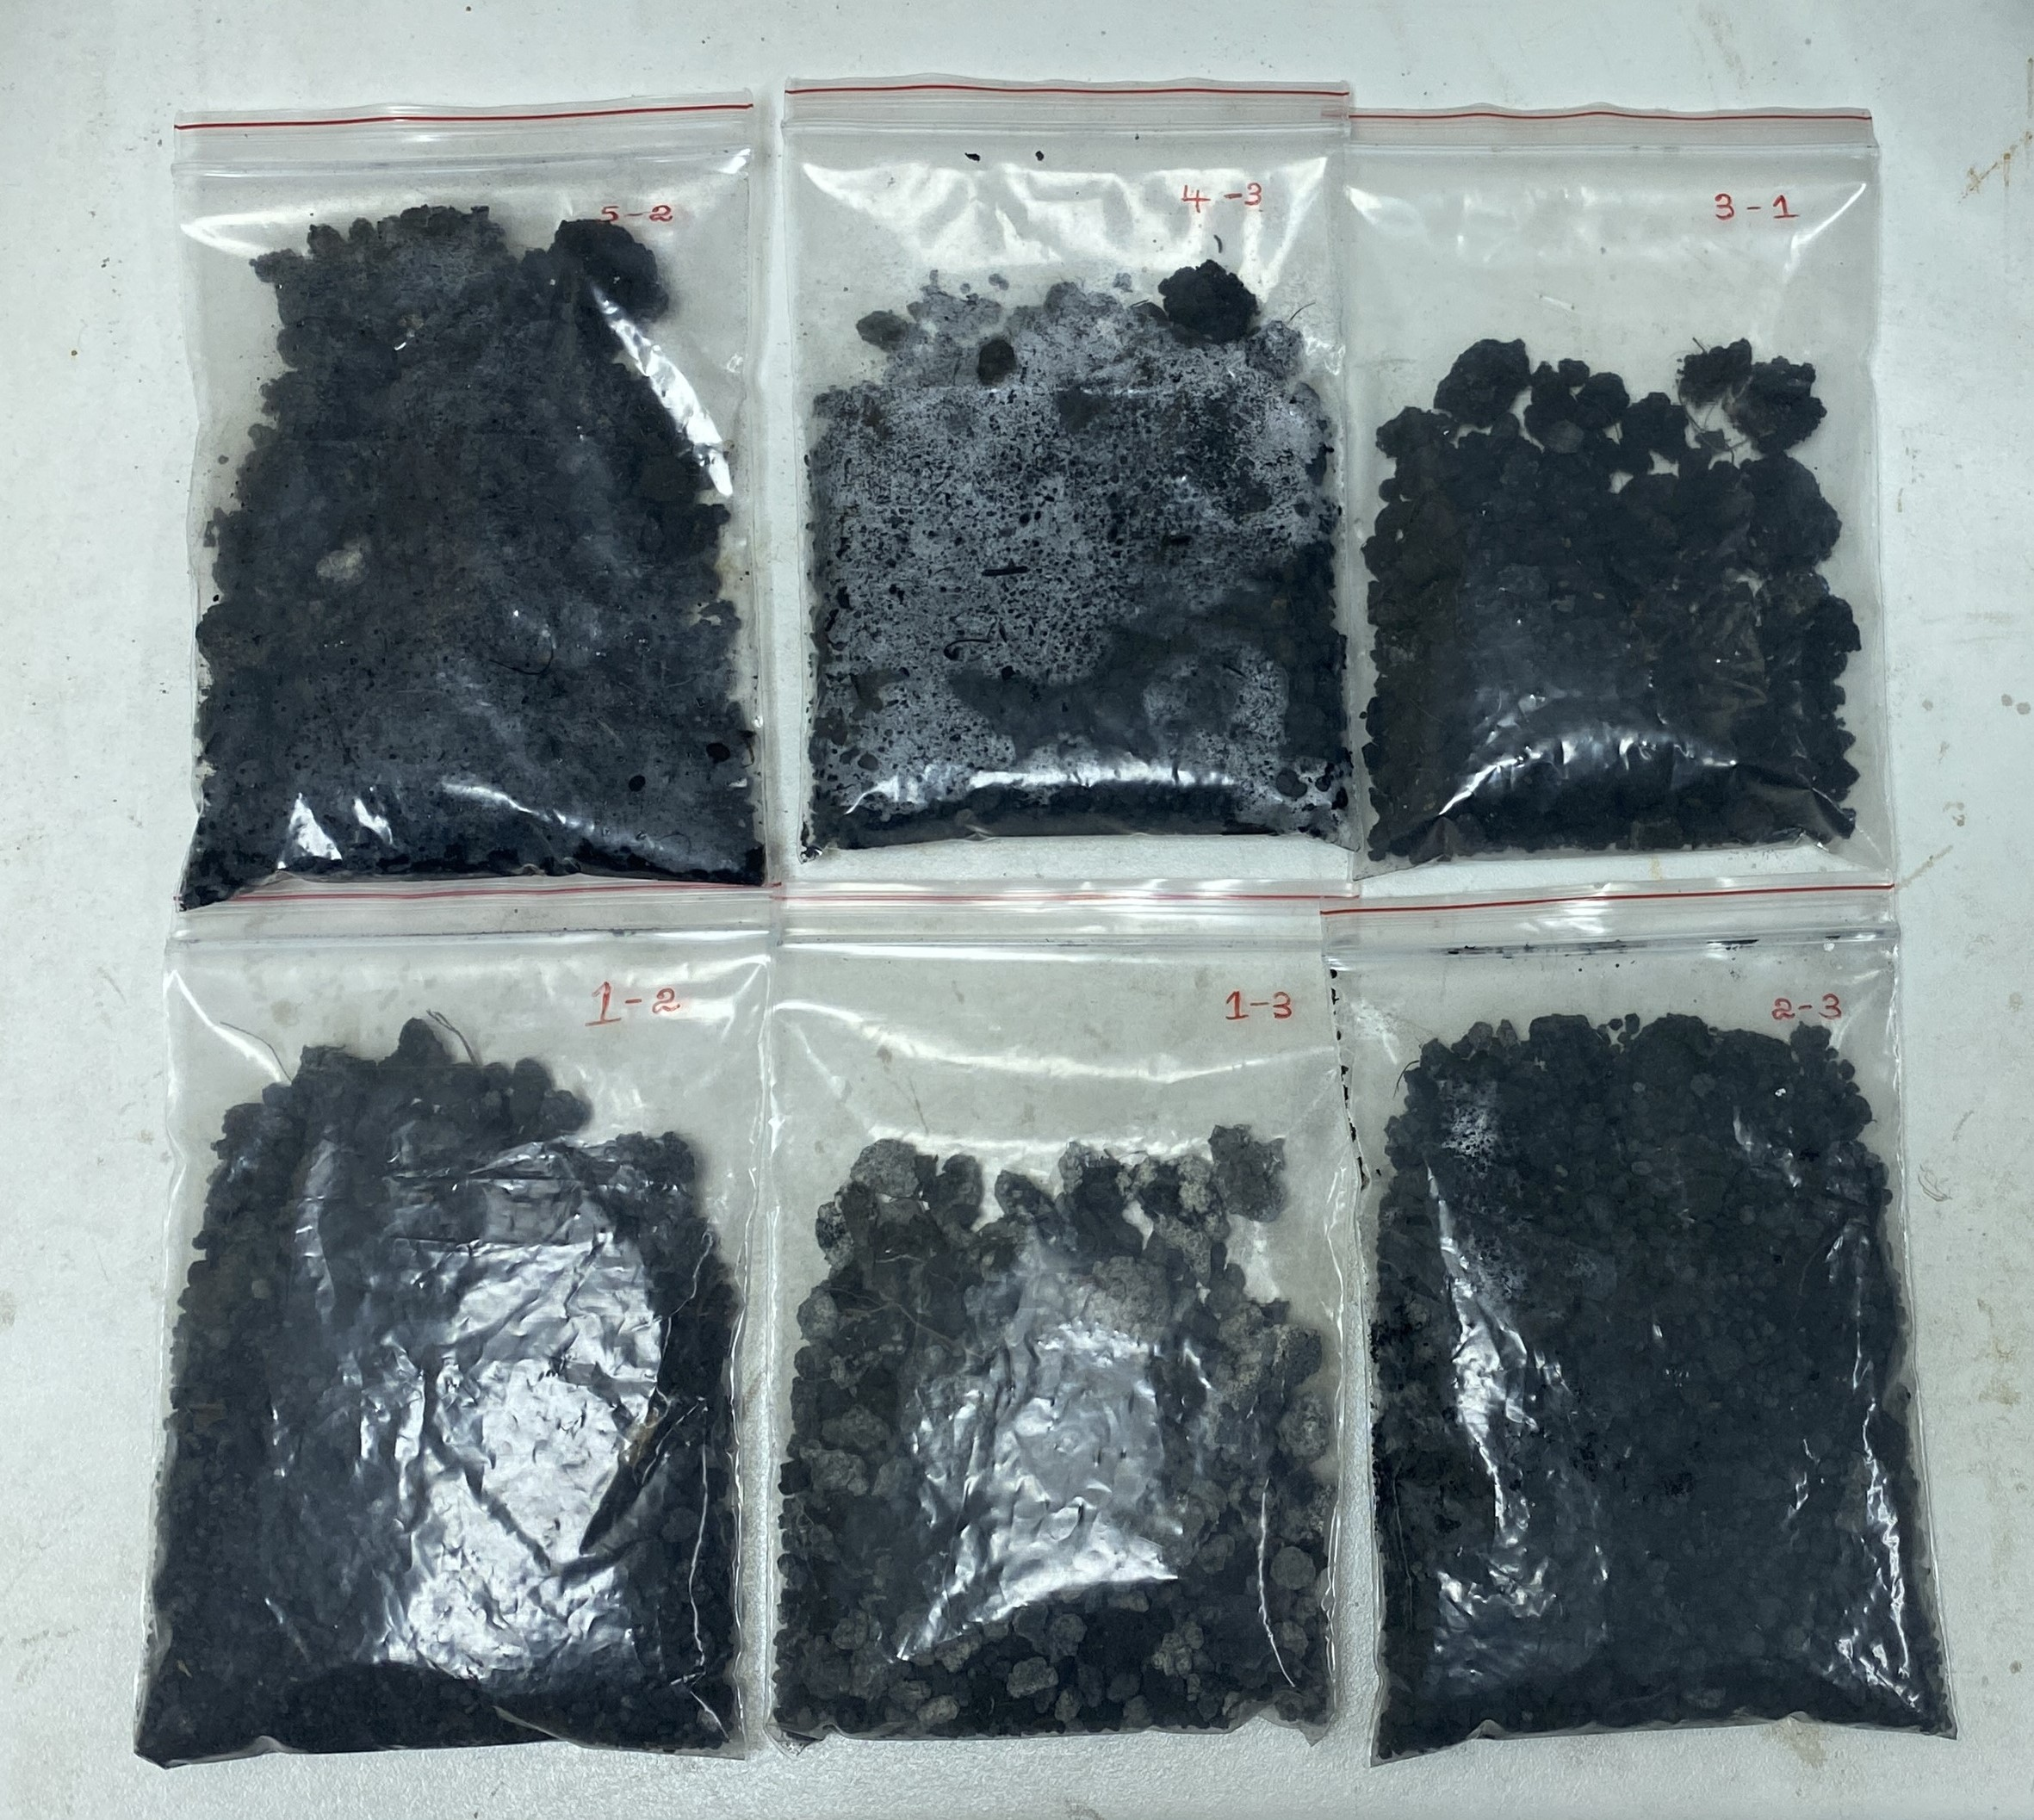
\includegraphics[width=0.6\linewidth]{results/Sample drying bed.jpg}
\caption{Sample collected from the different sample points at the drying bed}
\label{fig:Sample_dryingbed}
\end{figure}

\begin{figure}[H]
\centering
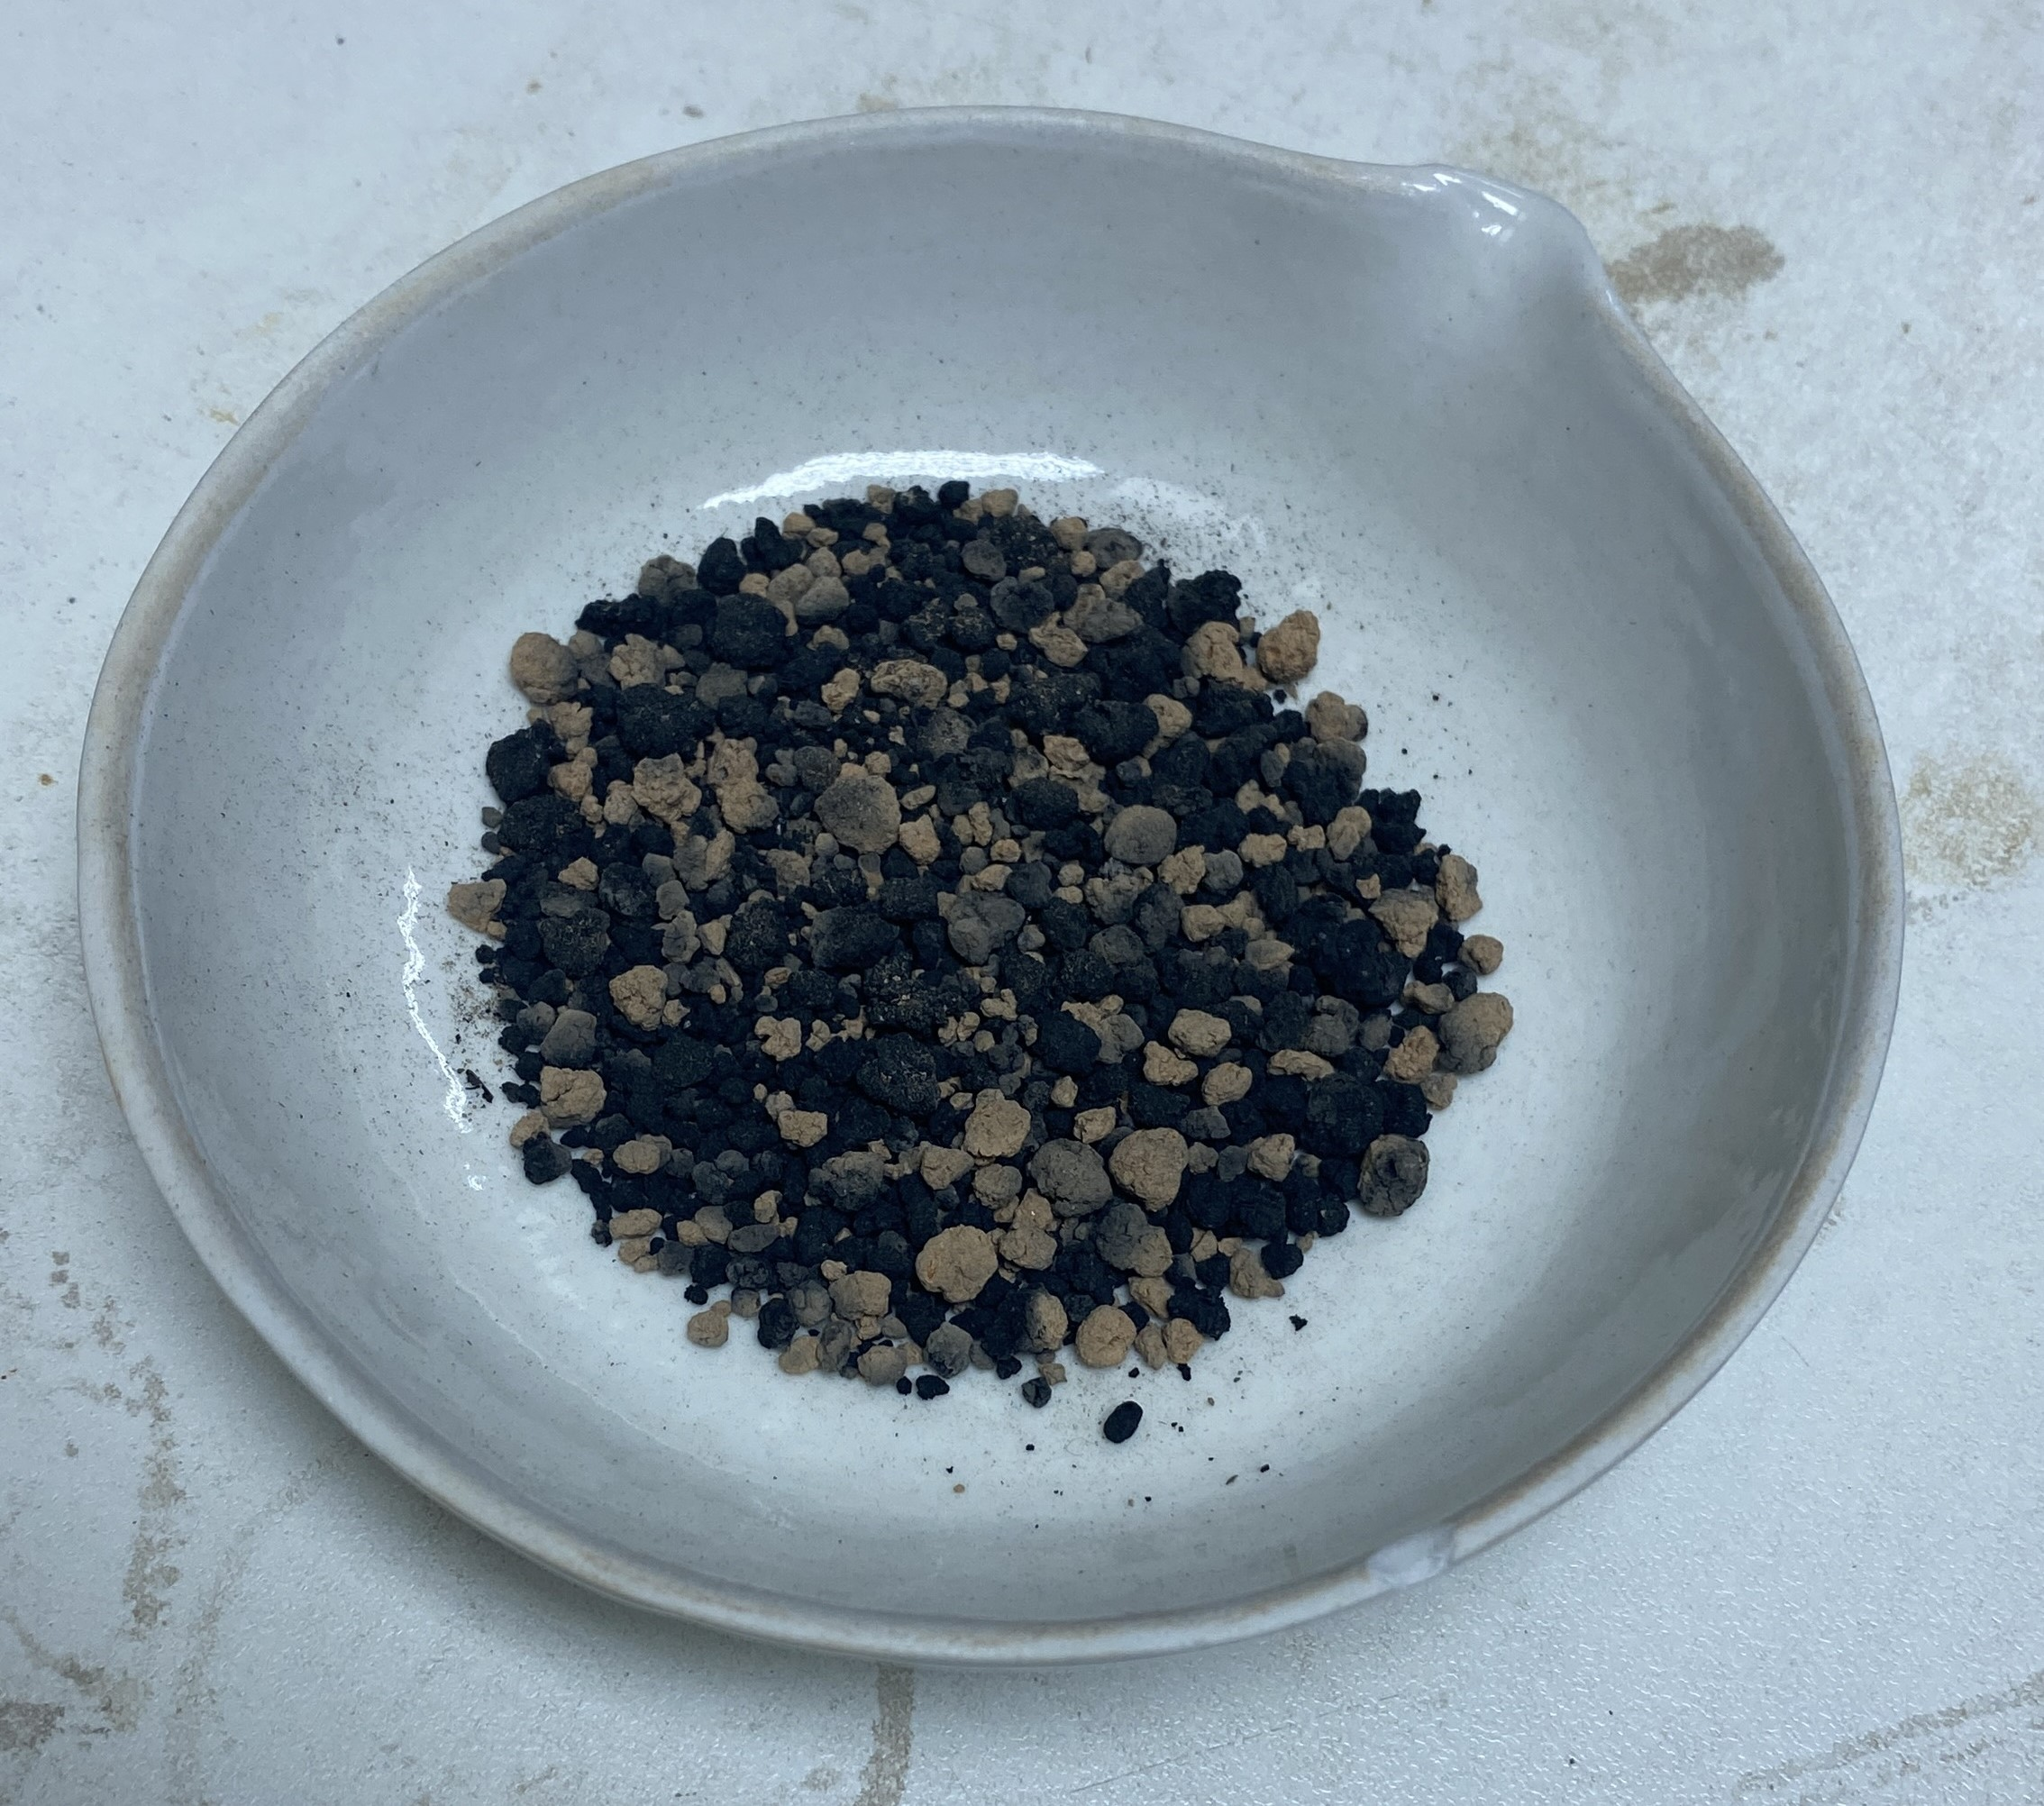
\includegraphics[width=0.6\linewidth]{results/SVMC sample.jpg}
\caption{\ac{SVMC} analyzed Sample after dried at 550 °C}
\label{fig:SVMC_sample}
\end{figure}

\subsection{Characteristics of wastewater}

\subsubsection{Daily Flow}
During the study period, the flow remained relatively stable, fluctuating between \numprint{13000} and \numprint{18000} \unit{m^3} from week 01 to week 13. After that, in between weeks 13 and 20 there was a notable increase in the flow in a range from \numprint{15000} to \numprint{37000} \unit{m^3}. After week 20, the flow stabilized again with a variation between \numprint{7000} and \numprint{18000} \unit{m^3}. The highest observed flow was \numprint{36722} \unit{m^3} in the week 16 and the lowest flow was \numprint{7224} \unit{m^3} in the week 30. The average flow during the period was \numprint{16671} \unit{m^3}. 

\begin{figure}[H]
    \centering

    \pgfplotstableread[col sep=comma]{results/flow_dataset.csv} \dataset

    \begin{tikzpicture}
        \begin{axis}[
            axis lines = left,
            scaled ticks=false,
            xlabel = Week,
            width = 13cm,
            height = 10cm,
            ylabel = Flow \unit{m^3},
            legend pos = south west,
            ymax=40000,
            ymin=5000,
            ymajorgrids=true, % Display only major gridlines
            yminorgrids=true, % Display minor gridlines
            extra y tick labels={}, % Empty labels for extra y ticks
            extra y ticks={7500,12500,17500,22500,27500,32500,37500}, % Add extra y ticks with minor tick values
            extra y tick style={grid=minor, grid style={dashed,gray!50}}, % Style for extra y ticks
        ]

            \addplot table[x index = {0}, y index = {1}]{\dataset};
        \end{axis}
         \draw [thick, black] (-2.5,-1.75) rectangle (13,9);
    \end{tikzpicture}

    \caption{Variation of the flow}
    \label{fig:flow_graph}
\end{figure}

\subsubsection{Temperature}
There was a slight difference in the temperature between the influent and effluent, as demonstrated in \Cref{fig:tempreature_graph}. Except for weeks 04, 16, 20, 25, and 30, the effluent temperature was higher than that of the influent for several weeks. During the $23^{rd}$ week, the temperature values of the influent and the effluent water were equal. During the week 16, the lowest temperature recorded for both the influent and effluent was 25.8 ℃, while the highest temperature recorded was 31.4 ℃ and 31.8 ℃ respectively, in the $12^{th}$ week.

\begin{figure}[H]
\centering

\pgfplotstableread[col sep=comma]{results/temp_vs_time_dataset.csv} \dataset

\begin{tikzpicture} \begin{axis}[
    ybar = 1.5pt,
    bar width = 4pt,
    width = 15cm,
    height = 10cm,
    axis lines = left,
    enlarge x limits = 0.02,
    ymin = 25, ymax = 32,
    ymajorgrids=true, % Display only major gridlines
                    yminorgrids=true, % Display minor gridlines
                    extra y tick labels={}, % Empty labels for extra y ticks
                    extra y ticks={25.5,26.5, ..., 31.5}, % Add extra y ticks with minor tick values
                    extra y tick style={grid=minor, grid style={dashed,gray!50}}, % Style for extra y ticks
    legend style={at={(0.5,-0.15)},
    anchor=north,legend columns=-1},
    xlabel = Sample Number,
    ylabel = Temperature (°C),
]
    \addplot table[x index = {0}, y index = {1}]{\dataset};
    \addplot table[x index = {0}, y index = {2}]{\dataset};
    
    \legend{Influent, Effluent}
\end{axis}
\draw [thick, black] (-2,-2.25) rectangle (14,9);
\end{tikzpicture}

\caption{Variation in temperature of influent and effluent}
\label{fig:tempreature_graph}
\end{figure}

\subsubsection{Hydrogen ion concentration (pH)}
\Cref{fig:ph_graph} shows a slight variation in the pH between the influent and effluent. The influent exhibits a pH range from 6.7 to 7.6, while the effluent exhibits a pH range from 6.8 to 7.7. During the study period, the influent pH indicates higher values than 7 except for weeks 14, 15, 16, 18 and 29, and the effluent pH indicates higher values than 7 in weeks expect 18, 24 and 29. The lowest and the highest pH value of influent and effluent noted was 6.7 in the week 29, 6.8 in the week 18, 7.6 in the week 3, and 7.7 in the week 6 respectively. There are 15 weeks during the period where the pH value of the effluent was higher than that of the influent.

\begin{figure}[H]
\centering

\pgfplotstableread[col sep=comma]{results/ph_dataset.csv} \dataset

\begin{tikzpicture} \begin{axis}[
    ybar = 1.5pt,
    bar width = 4pt,
    width = 15cm,
    height = 10cm,
    axis lines = left,
    enlarge x limits = 0.02,
    ymin = 6.6,
    ymax = 7.8,
     ymajorgrids=true, % Display only major gridlines
                    yminorgrids=true, % Display minor gridlines
                    extra y tick labels={}, % Empty labels for extra y ticks
                    extra y ticks={6.7,6.9, ..., 7.7}, % Add extra y ticks with minor tick values
                    extra y tick style={grid=minor, grid style={dashed,gray!50}}, % Style for extra y ticks
    legend style={at={(0.5,-0.15)},
    anchor=north,legend columns=-1},
    xlabel = Week,
    ylabel = pH,
]
    \addplot table[x index = {0}, y index = {1}]{\dataset};
    \addplot table[x index = {0}, y index = {2}]{\dataset};
    
    \legend{Influent, Effluent}
\end{axis}
\draw [thick, black] (-2.25,-2.25) rectangle (14.25,9);
\end{tikzpicture}

\caption{Variation in pH of influent and effluent}
\label{fig:ph_graph}
\end{figure}

\subsubsection{Biochemical Oxygen Demand (BOD$_5$)}
Sewage \ac{BOD} refers to the quantity of oxygen required for the biochemical degradation of biodegradable organic substances in aerobic conditions. The amount of oxygen absorbed during the cycle is directly correlated to the quantity of decomposable organic matter \cite{Prasad2020}. There was large variation in \ac{BOD5} between the influent and the effluent (\Cref{fig:bod_graph}). The influent and effluent \ac{BOD5} levels varied between 32 to 456 mg/l and 3 to 18 mg/l respectively. 

The highest value of 156 mg/l for the influent \ac{BOD5} was reported in week 19 and the lowest value of 32 mg/l was reported in the week 8. In week 8, the chart shows the lowest \ac{BOD5} level for influent and the highest \ac{BOD5} level for effluent. The tolerance limit for the short sea outfall outlined as 75 mg/l and during this study period effluent \ac{BOD5} concentration has not exceeded the tolerance limit \cite{CEA2022}. In week 8 and 21, the influent concentration of \ac{BOD5} was lower than the tolerance limit for short sea outfall outlined. The removal efficiency of \ac{BOD5} during this period varies from 43.75\% - 98.68\%, and the average removal efficiency was 93.55\%. During the performance evaluation conducted in 2016, the removal efficiency of \ac{BOD5} was reported as 94.12\% \cite{Danushika2016}.

\begin{figure}[H]
\centering

\pgfplotstableread[col sep=comma]{results/bod_dataset.csv} \dataset

\begin{tikzpicture} \begin{axis}[
    ybar = 1.5pt,
    bar width = 5pt,
    width = 15cm,
    height = 10cm,
    axis lines = left,
    enlarge x limits = 0.02,
    ymin = 0,
    ymax = 500,
     ymajorgrids=true, % Display only major gridlines
                    yminorgrids=true, % Display minor gridlines
                    extra y tick labels={}, % Empty labels for extra y ticks
                    extra y ticks={50,150, ...,450}, % Add extra y ticks with minor tick values
                    extra y tick style={grid=minor, grid style={dashed,gray!50}}, % Style for extra y ticks
    legend style={at={(0.5,-0.15)},
    anchor=north,legend columns=-1},
    xlabel = Week,
    ylabel = BOD (mg/l),
]
    \addplot table[x index = {0}, y index = {1}]{\dataset};
    \addplot table[x index = {0}, y index = {2}]{\dataset};
    
    \legend{Influent, Effluent}
\end{axis}
\draw [thick, black] (-2.25,-2.25) rectangle (14.25,9);
\end{tikzpicture}

\caption{Variation in BOD$_{5}$ of influent and effluent}
\label{fig:bod_graph}
\end{figure}


\subsubsection{Chemical Oxygen Demand (COD)}
\ac{COD} is the quantity of oxygen required for the oxidation of organic and some inorganic matter \cite{Prasad2020} and there was a large variation in \ac{COD} between the influent and the effluent. The influent and effluent \ac{COD} levels varied from 169 to 1647 mg/l and 23 to 76 mg/l respectively. During the first nine weeks, the \ac{COD} concentration of the influent was below 600 mg/l and was increased sharply in the week 10. However, in week 11, \ac{COD} concentration was decreased sharply and again showed a sharp increase in the week 12. During weeks 13 to 15, an increasing trend was visible with a sharp drop in the week 16. In the week 19, the \ac{COD} concentration was at its highest value for the period.  There was a gradual increment from weeks 25 to 27 and a gradual decrease was noted from weeks 27 to 29. During this study period, the effluent \ac{COD} concentration did not exceed the tolerance limit of 400 mg/l \cite{CEA2022}. The influent \ac{COD} concentration was below the tolerance limit of effluent for short sea outfall in 15 weeks and the removal efficiencies varied from 63.29\% to 97.21\% during this period. The average \ac{COD} removal efficiency reported was 86.90\% and the \ac{COD} removal efficiency reported during the performance evaluation done in 2016, the removal efficiency of \ac{COD} was 88.52\% \cite{Danushika2016}.

\begin{figure}[H]
\centering

\pgfplotstableread[col sep=comma]{results/cod_dataset.csv} \dataset

\begin{tikzpicture} \begin{axis}[
    ybar = 1.5pt,
    bar width = 5pt,
    width = 15cm,
    height = 10cm,
    axis lines = left,
    enlarge x limits = 0.02,
    ymin = 0,
    ymax = 1700,
     ymajorgrids=true, % Display only major gridlines
                    yminorgrids=true, % Display minor gridlines
                    extra y tick labels={}, % Empty labels for extra y ticks
                    extra y ticks={100,300, ..., 1700}, % Add extra y ticks with minor tick values
                    extra y tick style={grid=minor, grid style={dashed,gray!50}}, % Style for extra y ticks
    legend style={at={(0.5,-0.15)},
    anchor=north,legend columns=-1},
    xlabel = Week,
    ylabel = COD (mg/l),
]
    \addplot table[x index = {0}, y index = {1}]{\dataset};
    \addplot table[x index = {0}, y index = {2}]{\dataset};
    
    \legend{Influent, Effluent}
\end{axis}
\draw [thick, black] (-2.25,-2.25) rectangle (14.25,9);
\end{tikzpicture}

\caption{Variation of COD of influent and effluent }
\label{fig:COD_graph}
\end{figure}


\subsubsection{Total Suspended Solids (TSS)}
\Cref{fig:tss_graph} shows a slight variation in \ac{TSS} between the influent and the effluent during this period. The influent and effluent concentration of \ac{TSS} varied from 74 to 1438 mg/l and 4 to 28 mg/l respectively. The highest and the lowest concentrations of influent \ac{TSS} was observed in the weeks 19 and 21. The concentrations of \ac{TSS} observed during the first 9 weeks were below 450 mg/l and after in $10^{th}$ week, a sharp increase in the influent \ac{TSS} concentration was observed.

From weeks 10 to 19, the influent \ac{TSS} concentration fluctuated and, in the week 19, \ac{TSS} concentration of influent reached its peak, followed by a sharp decrease in next two weeks. During the last 9 weeks, the \ac{TSS} concentration did not exceed 700 mg/l.  During the weeks 6, 20 and 24, the lowest effluent concentration of \ac{TSS} was observed, and in week $9^{th}$ week, the highest value for the effluent \ac{TSS} was reported. The removal efficiency for this period varied from 75.99\% - 99.32\% and average removal efficiency was found as 95.28\%. However, during the performance evaluation conducted in 2016, the removal efficiency of \ac{TSS} has reported as 97.05\% \cite{Danushika2016}.

\begin{figure}[H]
\centering

\pgfplotstableread[col sep=comma]{results/tss_dataset.csv} \dataset

\begin{tikzpicture} \begin{axis}[
    ybar = 1.5pt,
    bar width = 5pt,
    width = 15cm,
    height = 10cm,
    axis lines = left,
    enlarge x limits = 0.02,
    ymin = 0,
    ymax = 1500,
    ymajorgrids=true, % Display only major gridlines
                    yminorgrids=true, % Display minor gridlines
                    extra y tick labels={}, % Empty labels for extra y ticks
                    extra y ticks={100,300, ..., 1500}, % Add extra y ticks with minor tick values
                    extra y tick style={grid=minor, grid style={dashed,gray!50}}, % Style for extra y ticks
    legend style={at={(0.5,-0.15)},
    anchor=north,legend columns=-1},
    xlabel = Week,
    ylabel = TSS (mg/l),
]
    \addplot table[x index = {0}, y index = {1}]{\dataset};
    \addplot table[x index = {0}, y index = {2}]{\dataset};
    
    \legend{Influent, Effluent}
\end{axis}
\draw [thick, black] (-2.25,-2.25) rectangle (14.25,9);
\end{tikzpicture}

\caption{Variation in TSS of influent and effluent}
\label{fig:tss_graph}
\end{figure}




\subsubsection{Oil and Grease Concentration}

One common type of pollutant found in water and wastewater is "Oil and Grease". Organic compounds of the \ac{OG} group have an extremely low affinity for water. Substances commonly categorized as consists of hydrocarbons, soaps, fatty acids, waxes and lipids \cite{Pintor2016}. \Cref{fig:OG_graph} shows a large variation between the influent and the effluent in \ac{OG} concentration. The variation of the \ac{OG} in the influent and the effluent was observed to be 7.5 to 26.8 mg/l and 0 to 1.1 mg/l respectively. In several weeks, the influent \ac{OG} concentration was higher than 10 mg/l and the average concentration was 15.16 mg/l. In first 5 weeks, concentration varied between 10 to 15 mg/l and after, a sharp increase was noted in the $6^{th}$ week.

During weeks 6 to 9, the concentration of \ac{OG} varied between 15 to 25 mg/l.  The highest and the lowest concentration of influent was observed in weeks 14 and 21. Both weeks 16 and 17 showed equal concentration of 12.5 mg/l. The concentration of effluent did not exceed the tolerance limit for short sea outfall outlined as 12 mg/l and in the $8^{th}$ week, \ac{OG} concentration of influent too was lower than the tolerance limit \cite{CEA2022}. The removal efficiency of the \ac{OG} was found to be 97.04\%.\\

\begin{figure}[H]
\centering

\pgfplotstableread[col sep=comma]{results/oil_and_grease_dataset.csv} \dataset

\begin{tikzpicture} \begin{axis}[
    ybar = 1.5pt,
    bar width = 5pt,
    width = 15cm,
    height = 10cm,
    axis lines = left,
    enlarge x limits = 0.03,
    ymin = 0,
    ymajorgrids=true, % Display only major gridlines
                    yminorgrids=true, % Display minor gridlines
                    extra y tick labels={}, % Empty labels for extra y ticks
                    extra y ticks={2.5,7.5,12.5,17.5,22.5}, % Add extra y ticks with minor tick values
                    extra y tick style={grid=minor, grid style={dashed,gray!50}}, % Style for extra y ticks
    legend style={at={(0.5,-0.15)},
    anchor=north,legend columns=-1},
    xlabel = Week,
    ylabel = Oil \& Grease (mg/l),
]
    \addplot table[x index = {0}, y index = {1}]{\dataset};
    \addplot table[x index = {0}, y index = {2}]{\dataset};
    
    \legend{Influent, Effluent}
\end{axis}
\draw [thick, black] (-2,-2.25) rectangle (14,9);
\end{tikzpicture}

\caption{Variation of Oil and Grease}
\label{fig:OG_graph}
\end{figure}


\subsubsection{Ortho Phosphate (as P)}
During the study period, as depicted in the \Cref{fig:OrthoP_graph}, several weeks showed that the concentration of ortho-phosphate is more than 0.4 mg/l. The highest observed ortho-phosphate concentration of the influent was 0.8 mg/l during the weeks 10, 22 and 30, and the lowest orthophosphate concentration of influent noted was 0.1 mg/l in $17^{th}$ week. During first 9 weeks, the concentration varied between 0.4 and 0.8 mg/l and after the $13^{th}$ week, the concentration of influent was decreased to 0.2 mg/l.

From weeks 14 to 18, the concentration of influent varied from 0.1 to 0.3 mg/l. while last 12 weeks starting from $19^{th}$ week, showed that the influent ortho-phosphate concentration lied between 0.4 and 0.8 mg/l. Considering the effluent ortho-phosphate concentration, first 4 weeks showed equal values and since then there was a gradual increase between weeks 8 and 10. A sharp decrease of the concentration was observed for the weeks 8 to 11. From week 11 to 30, the concentration was observed below 0.2 mg/l and during the study period, the ortho-phosphate concentration of both influent and the effluent did not exceed the tolerance limit for short sea outfall outlined as 5.0 mg/l \cite{CEA2022}. 
\begin{figure}[H]
\centering

\pgfplotstableread[col sep=comma]{results/ortho_posphate_dataset.csv} \dataset

\begin{tikzpicture} \begin{axis}[
    ybar = 1.5pt,
    bar width = 5pt,
    width = 15cm,
    height = 10cm,
    axis lines = left,
    enlarge x limits = 0.03,
    ymin = 0,
    ymajorgrids=true, % Display only major gridlines
                    yminorgrids=true, % Display minor gridlines
                    extra y tick labels={}, % Empty labels for extra y ticks
                    extra y ticks={0.15, 0.25,0.35,0.45,0.55,0.65,0.75}, % Add extra y ticks with minor tick values
                    extra y tick style={grid=minor, grid style={dashed,gray!50}}, % Style for extra y ticks
    legend style={at={(0.5,-0.15)},
    anchor=north,legend columns=-1},
    xlabel = Week,
    ylabel = Ortho Posphate (\unit{mg/l}),
]
    \addplot table[x index = {0}, y index = {1}]{\dataset};
    \addplot table[x index = {0}, y index = {2}]{\dataset};
    
    \legend{Influent, Effluent}
\end{axis}
\draw [thick, black] (-2,-2.25) rectangle (14,9);
\end{tikzpicture}

\caption{Variation of Ortho Phosphate of influent and effluent }
\label{fig:OrthoP_graph}
\end{figure}




\subsubsection{Fluoride (as F)}
\Cref{fig:Fluo_graph} shows a considerable variation of concentration of Fluoride (as F) in the influent and the effluent. In the first four weeks, the influent concentration was reported below 0.3 mg/l, while the lowest concentration of 0.2 mg/l was observed in the $19^{th}$ week.  Thereafter, the concentration of Fluoride of the influent was noted as 0.5 mg/l, and there was a gradual decrease between weeks 20 to 22.

During weeks 23 and 24, the concentration was 0.4 mg/l, and then a gradual increase was observed from week 24. Both weeks 26 and 27 indicated the exact value of 0.6 mg/l for the concentration of the influent and there was a decreasing trend visible from week 27 to week 29.  The highest concentration of the influent of 0.7 mg/l was observed during the last week of the study period. The Fluoride concentration of the effluent showed values less than or equal to 0.2 mg/l during the study period. Importantly, both influent and effluent concentrations did not exceed the tolerance limit outlined as 2 mg/l \cite{CEA2022}.


\begin{figure}[H]
\centering

\pgfplotstableread[col sep=comma]{results/fluoride_dataset.csv} \dataset
\begin{tikzpicture} \begin{axis}[
    ybar = 2pt,
    bar width = 5pt,
    width = 15cm,
    height = 10cm,
    axis lines = left,
    % enlargelimits=0.01,
    xmax = 31,
    xmin = 15,
    ymin = 0.05,
    ymajorgrids=true, % Display only major gridlines
                    yminorgrids=true, % Display minor gridlines
                    extra y tick labels={}, % Empty labels for extra y ticks
                    extra y ticks={0.15, 0.25,0.35,0.45,0.55,0.65}, % Add extra y ticks with minor tick values
                    extra y tick style={grid=minor, grid style={dashed,gray!50}}, % Style for extra y ticks
    legend style={at={(0.5,-0.15)},
    anchor=north,legend columns=-1},
    ylabel = Fluoride (mg/l),
    xtick=data,
]
    \addplot table[x index = {0}, y index = {1}]{\dataset};
    \addplot table[x index = {0}, y index = {2}]{\dataset};
    \legend{Influent, Effluent}
\end{axis}
\draw [thick, black] (-2,-2.25) rectangle (14,9);
\end{tikzpicture}

\caption{Variation of Fluoride (as F) of influent and effluent }
\label{fig:Fluo_graph}
\end{figure}


\subsubsection{BOD/COD Ratio}
Biodegradability was calculated using the ratio of \ac{BOD5} and \ac{COD} and as shown in the \Cref{fig:BOD/COD_graph}, for the influent, the ratio between \ac{BOD5} and \ac{COD} lied between 0.18 to 0.56. For the effluent \ac{BOD5}/\ac{COD} ratio was ranged between 0.08 to 0.36. In the majority number of weeks,\ac{BOD5}/ \ac{COD} ratio of the influent showed values below 0.50 except for weeks 14 and 27. Considering the effluent, the majority of the time, the \ac{BOD5}/\ac{COD} ratio was below 0.30 except for weeks 8, 10, 14, and 28. The highest and the lowest ratios were 0.56 in week 14 and 0.18 in week 8, respectively. The average value of the ratio observed was 0.39 for the influent. The highest and lowest values observed for the effluent were 0.36 in week 8 and 0.08 in week 6, with an average of 0.18. 
\begin{figure}[H]
\centering

\pgfplotstableread[col sep=comma]{results/bod_cod_ratio_dataset.csv} \dataset

\begin{tikzpicture} \begin{axis}[
    ybar = 1.5pt,
    bar width = 4pt,
    width = 15cm,
    height = 10cm,
    axis lines = left,
    enlarge x limits = 0.02,
    ymin = 25, ymax = 32,
    legend style={at={(0.5,-0.15)},
    anchor=north,legend columns=-1},
    xlabel = Sample Number,
    ylabel = BOD$_5$ / COD,
    ymax=0.6, ymin=0,
    ymajorgrids=true, % Display only major gridlines
                    yminorgrids=true, % Display minor gridlines
                    extra y tick labels={}, % Empty labels for extra y ticks
                    extra y ticks={0.15, 0.25,0.35,0.45,0.55}, % Add extra y ticks with minor tick values
                    extra y tick style={grid=minor, grid style={dashed,gray!50}}, % Style for extra y ticks
]
    \addplot table[x index = {0}, y index = {1}]{\dataset};
    \addplot table[x index = {0}, y index = {2}]{\dataset};
    
    \legend{Influent, Effluent}
\end{axis}
\draw [thick, black] (-2,-2.25) rectangle (14,9);
\end{tikzpicture}

\caption{Variation in biodegradability of influent and effluent}
\label{fig:BOD/COD_graph}
\end{figure}



\subsection{Removal Efficiencies}
According to \Cref{tab:average_removal_efficiency_table}, the highest average \ac{BOD5} removal efficiency was indicated in November month as 97.34\%, and the lowest efficiency was indicated as 82.49\% in July. There was an average efficiency during the period indicated as 93.55\%. The highest average \ac{COD} removal efficiency was indicated in July, and the lowest value was indicated in June during the study period. As shown in \Cref{tab:average_removal_efficiency_table}, \ac{TSS} removal efficiency varies from 91.46\% to 97.80\%.  Moreover, the average removal efficiencies of \ac{OG}, Ortho-phosphate, and fluoride were indicated as 97.04\%, 79.08\%, and 68.04\%, respectively. During the period, the orthophosphate and fluoride removal efficiencies increased gradually.

\begin{table}[H]
    \caption{Average removal efficiencies of different parameters}
    \begin{tabular}{|>{\raggedright\arraybackslash}p{0.135\linewidth}|>{\centering\arraybackslash}p{0.11\linewidth}|>{\centering\arraybackslash}p{0.11\linewidth}|>{\centering\arraybackslash}p{0.11\linewidth}|>{\centering\arraybackslash}p{0.11\linewidth}|>{\centering\arraybackslash}p{0.12\linewidth}|>{\centering\arraybackslash}p{0.105\linewidth}|}
        \hline
        \textbf{Month}     & \textbf{BOD$_5$  (\%)} & \textbf{COD (\%)}& \textbf{TSS (\%)} & \textbf{Oil \& Grease (\%)} & \textbf{Ortho-phosphate (\%)} & \textbf{Fluoride (as F) (\%)} \\
        \hline
        \textbf{June}      & 94.24                                                        & 95.78             & 96.73             & 95.78                  & -                        & -                        \\
        \textbf{July}      & 82.49                                                        & 98.36             & 91.46             & 98.36                  & 79.17                    & -                        \\
        \textbf{August}    & 94.56                                                        & 97.53             & 92.71             & 97.53                  & 73.50                    & -                        \\
        \textbf{September} & 96.04                                                        & 97.35             & 95.74             & 97.35                  & 67.50                    & 45.83                    \\
        \textbf{October}   & 94.43                                                        & 96.50             & 96.54             & 96.50                  & 88.27                    & 61.67                    \\
        \textbf{November}  & 97.34                                                        & 96.69             & 97.80             & 96.69                  & 82.00                    & 78.97                    \\
        \textbf{December}  & 92.37                                                        & 96.54             & 96.64             & 96.54                  & 85.48                    & 75.86                    \\
        \hline
        \hline
        \textbf{Min}       & 43.75                                                        & 63.29             & 75.44             & 94.20                  & 50.00                    & 45.83                    \\
        \textbf{Max}       & 98.68                                                        & 97.21             & 99.32             & 100.00                 & 92.59                    & 88.33                    \\
        \textbf{Average}   & 93.55                                                        & 86.95             & 95.28             & 97.04                  & 79.08                    & 68.04                    \\
        \textbf{SD}        &  9.91                                                            &  8.84                & 5.26                  &  1.38                       & 9.92                          &  14.80\\
     \hline
    \end{tabular}
    \label{tab:average_removal_efficiency_table}
\end{table}

\subsection{Correlations}
The consistency of correlations between different measures of organic content depends mostly on the characteristics of the wastewater and its origin. Regression analysis was used to assess the relationship between influent \ac{BOD5} and influent \ac{TSS}, as well as the relationship between removal efficiency of \ac{BOD5} and removal efficiency of \ac{TSS}. Due to the rapidness of \ac{TSS} tests, these correlations can be highly beneficial as \ac{BOD5} measurements require 5 days. After establishing the correlation, \ac{TSS} monitoring can be effectively utilized for treatment plant operation \cite{Kumar2010}.

\begin{table}
    \centering
    \caption{Correlations between $BOD_5$ and TSS}
    \begin{tabular}{|>{\raggedright\arraybackslash}p{5.5cm}|p{5.5cm}|p{4 cm}|}
    \hline
          & Expression & Correlation coefficient\\
          \hline
         Variation between influent BOD (y) and TSS (x) & $$y = 57.6499 + 0.38406x $$ & $$ r = 0.8187 $$ \\
         \hline
         Variation between removal efficiency of BOD (y) and removal efficiency of TSS (x) & $$y = -0.0095 + 0.9940 x$$& $$r = 0.6718$$\\
         \hline
    \end{tabular}
    \label{tab:BOD_TSS_correlations}
\end{table}

\newpage
\subsection{Sludge Management}

\subsubsection{Belt Filter Press Efficiency}
From December to February, the belt filter press efficiency was measured using the solid content of the dewatered sludge cake. During the time period, the solid content of the sludge cake varied from 11.00\% to 14.50\%. The highest solid content of 14.06\% was observed on $01^{st}$ December 2023, and the lowest solid content of 11.32\% was noted on $08^{th}$ January 2024.

The \ac{TSS} concentration of the sludge storage tank and the return water from the belt press is shown in \Cref{fig:Solid_Recovered_graph}. Sludge storage tank has a \ac{TSS} value between \numprint{20000} mg/l and \numprint{30000} mg/l. Return water \ac{TSS} concentration varies between 80 mg/l and 300 mg/l. The percentage of solid recovery is over 99\% for the study period.

\begin{figure}[H]
\centering

\pgfplotstableread[col sep=comma] {results/ds_content_dataset.csv} \dataset
                \begin{tikzpicture}
                \begin{axis}[
                ybar,
                bar width = 10pt,
                    date coordinates in=x,
                    axis lines = left,
                    table/col sep=comma,
                    xlabel = Date,
                    xlabel style={
                        at={(0.5,-11ex)}
                    },
                    xticklabel style={
                        rotate=45,
                        anchor=near xticklabel,
                    },
                    xtick=data,
                    xticklabel=\year-\month-\day,
                    width = 15cm,
                    height = 9cm,
                    ylabel = Solid Content (\%),
                    ymax=15,
                    ymin=10,
                     xmin = 2023-11-25,
                    xmax = 2024-02-10,
                    ymajorgrids=true, % Display only major gridlines
                    yminorgrids=true, % Display minor gridlines
                    extra y tick labels={}, % Empty labels for extra y ticks
                    extra y ticks={10.50, 11.50,12.5,13.5,14.50}, % Add extra y ticks with minor tick values
                    extra y tick style={grid=minor, grid style={dashed,gray!50}}, % Style for extra y ticks
                    ]
                    \addplot  table[x=Date,y=Solid content] {\dataset};;
                \end{axis}
                \draw [thick, black] (-2,-2.8) rectangle (14,8);
            \end{tikzpicture}

\caption{Variation in solid content of the dewatered sludge}
\label{fig:ds_content_graph}
\end{figure}


\begin{figure}[H]
\centering

\pgfplotstableread[col sep=comma] {results/Solid_recovered_dataset.csv} \dataset
                \begin{tikzpicture}
                \begin{axis}[
                    ybar = 4pt,
                    bar width = 10pt,
                    date coordinates in=x,
                    axis lines = left,
                    table/col sep=comma,
                    scaled ticks=false,
                    xlabel = Date,
                    xlabel style={
                        at={(0.5,-11ex)}
                    },
                    ylabel style={
                        at={(-0.125, 0.5)}
                    },
                    xticklabel style={
                        rotate=45,
                        anchor=near xticklabel,
                    },
                    xtick=data,
                    xticklabel=\year-\month-\day,
                    legend style={at={(0.4,-0.4)},
                    anchor=north,legend columns=-1},
                    width = 15cm,
                    height = 9cm,
                    ylabel = TSS (mg/l),
                    ymax=30000,
                    ymin=0,
                    xmin = 2023-11-25,
                    xmax = 2024-02-10,
                    ymajorgrids=true, % Display only major gridlines
                    yminorgrids=true, % Display minor gridlines
                    extra y tick labels={}, % Empty labels for extra y ticks
                    extra y ticks={2500, 7500, 12500, 17500, 22500, 27500}, % Add extra y ticks with minor tick values
                    extra y tick style={grid=minor, grid style={dashed,gray!50}}, % Style for extra y ticks
                    ]
                    \addplot table[x index = {0}, y index = {1}]{\dataset};
                    
                    \addplot table[x index = {0}, y index = {2}]{\dataset};

    \legend{Return water TSS, Sludge tank TSS}
                \end{axis}
                \draw [thick, black] (-2.5,-3.85) rectangle (14,9);
            \end{tikzpicture}

\caption{Variation of TSS in Sludge storage tank and the return water}
\label{fig:Solid_Recovered_graph}
\end{figure}

\subsubsection{Sludge Drying Bed Performance}
\Cref{fig:mc_differentpoints__graph} shows the variation of the moisture content of different sampling points during the period. On $12^{th}$ December 2023, sampling points 1, 2, 3, and 4 had moisture contents ranged between 61\% and 68\%, and sample point 5 had the lowest moisture content. The average moisture content on $12^{th}$ December was indicated as 62.04\%. On $13^{th}$ January 2024, the lowest moisture content of the dried sludge was indicated as 26.16\% at sample point 4, and the highest moisture content was 52.75\% at sample point 1. The Moisture content of the other samples varied between 38\% and 46\%. The average moisture content of these samples was 41.27\%

On $29^{th}$ January 2024, all the samples showed a moisture content less than 58\% while the highest and the lowest moisture content were observed in samples 5 and 1, respectively. The average moisture content was as 48.61\%, and on $16^th$ February, sample point 2 had the highest moisture content and sample 4 had the lowest moisture content. The moisture content of the other three samples varied between 36\% and 42\%. The average moisture content among different sampling points on $16^th$ February was observed as 38.52\%

\begin{figure}[H]
\centering

\pgfplotstableread[col sep=comma]{results/sludge_moisture_different_point_dataset.csv} \dataset
                \begin{tikzpicture}
                \begin{axis}[
                    ybar = 1.5pt,
                    bar width = 9pt,
                    enlarge x limits={abs=0.8}, % Adjust spacing between bars
                    date coordinates in=x,
                    axis lines = left,
                    table/col sep=comma,
                    xlabel = Time (Date),
                    xlabel style={
                        at={(0.5,-11ex)}
                    },
                    xticklabel style={
                        rotate=45,
                        anchor=near xticklabel,
                    },
                    xtick=data,
                    xticklabel=\year-\month-\day,
                    width = 15cm,
                    height = 10cm,
                    ylabel = Moisture Content (\%),
                    legend style={at={(0.5,-0.4)},
                    anchor=north,legend columns=-1},
                    ymin = 0,
                    ymax = 70,
                    enlarge x limits = 0.10,
                    ymajorgrids=true, % Display only major gridlines
                    yminorgrids=true, % Display minor gridlines
                    extra y tick labels={}, % Empty labels for extra y ticks
                    extra y ticks={5, 15, ..., 65}, % Add extra y ticks with minor tick values
                    extra y tick style={grid=minor, grid style={dashed,gray!50}}, % Style for extra y ticks
                    ]
                    \addplot table[x index = {0}, y index = {1}] {\dataset};
                    \addplot table[x index = {0}, y index = {2}] {\dataset};
                    \addplot table[x index = {0}, y index = {3}] {\dataset};
                    \addplot table[x index = {0}, y index = {4}] {\dataset};
                    \addplot table[x index = {0}, y index = {5}] {\dataset};

                    \legend{sample 1$S_5$, sample 2$S_5$, sample 3$S_5$, sample 4$S_5$, sample 5$S_5$};

                \end{axis}
                \draw [thick, black] (-2,-4.25) rectangle (14,9);
            \end{tikzpicture}

\caption{Variation in moisture content in different sampling points at sludge drying bed}
\label{fig:mc_differentpoints__graph}
\end{figure}

\Cref{fig:mc_dewatered_dried_graph} showed the average moisture content of the dewatered sludge and the dried sludge. At the initial discharge stage, the dewatered sludge had the minimum moisture content compared to the other times, while the dried sludge behaved in the opposite way with a higher moisture content compared to the other times.

During the second discharge of sludge, the dewatered sludge moisture content was observed as 88.68\% and the dried sludge moisture content was noted as 41.27\%. The removal percentage of moisture content during the drying process was 53.47\% during this time (\Cref{table:removal_precentage}). In the third discharge of sludge, the dewatered sludge and the dried sludge moisture content were 86.63\% and 48.61\%, respectively. The removal percentage of moisture content during the drying process was found to be as 43.89\% during this time. Also, for this time period, the highest removal percentage was obtained for the fourth discharge stage (\Cref{table:removal_precentage}).

\begin{figure}[H]
\centering

\pgfplotstableread[col sep=comma]{results/mc_dewatered_dried_dataset.csv} \dataset

\begin{tikzpicture}
  \begin{axis}[
   ybar = 4pt,
    bar width = 10pt,
   axis lines = left,
   xlabel = Discharge round,
   width = 15cm,
   height = 10cm,
    ylabel =    Moisture content (\%),
     enlarge x limits = 0.05,
     xtick=data,
     ymax=90, ymin=35,
    ymajorgrids=true, % Display only major gridlines
                    yminorgrids=true, % Display minor gridlines
                    extra y tick labels={}, % Empty labels for extra y ticks
                    extra y ticks={45,55,65,75,85}, % Add extra y ticks with minor tick values
                    extra y tick style={grid=minor, grid style={dashed,gray!50}}, % Style for extra y ticks
                    legend style={at={(0.5,-0.15)},
    anchor=north,legend columns=-1},
    ]
    \addplot table[x index = {0}, y index = {1}]{\dataset};
    \addplot table[x index = {0}, y index = {2}]{\dataset};

    \legend{Dewatered sludge, Dried sludge}
  \end{axis}
  \draw [thick, black] (-2,-2.2) rectangle (14,9);
\end{tikzpicture}

\caption{Variation in average moisture content of dewatered and dried sludge}
\label{fig:mc_dewatered_dried_graph}
\end{figure}